%% This is file `DEMO-TUDaThesis-de.tex' version 4.05 (2025-11-13),
%% it is part of
%% TUDa-CI -- Corporate Design for TU Darmstadt
%% ----------------------------------------------------------------------------
%%
%% Copyright (C) 2018--2025 by Marei Peischl <marei@peitex.de>
%%
%% ============================================================================
%% This work may be distributed and/or modified under the
%% conditions of the LaTeX Project Public License, either version 1.3c
%% of this license or (at your option) any later version.
%% The latest version of this license is in
%% http://www.latex-project.org/lppl.txt
%% and version 1.3c or later is part of all distributions of LaTeX
%% version 2008/05/04 or later.
%%
%% This work has the LPPL maintenance status `maintained'.
%%
%% The current maintainer of this work is
%%   Marei Peischl <tuda-ci@peitex.de>
%%
%% The development repository can be found at
%% https://github.com/tudace/tuda_latex_templates
%% Please use the issue tracker for feedback!
%%
%% If you need a compiled version of this document, have a look at
%% http://mirror.ctan.org/macros/latex/contrib/tuda-ci/doc
%% or at the documentation directory of this package (if installed)
%% <path to your LaTeX distribution>/doc/latex/tuda-ci
%% ============================================================================
%%
% !TeX program = lualatex
%%

% PDF/A über pdfmanagement
% Vermutlich temporärer Workaround für eine Inkompatibilität mit dem tagging-project  https://github.com/tudace/tuda_latex_templates/issues/521
% \DocumentMetadata{
\RequirePackage{pdfmanagement}
\SetKeys[document/metadata]{
	pdfstandard=a-2b,
	pdfversion=1.7,% 2.0 geht auch, aber dann geht kein PDF/A-2b
	lang=de,
}

\documentclass[
	german,% Hauptsprache als globale Option, früher war ngerman notwendig
	accentcolor=9c,% Auswahl der Akzentfarbe
	ruledheaders=section,% Ebene bis zu der die Überschriften mit Linien abgetrennt werden
	class=report,% Basisdokumentenklasse. Wählt die korrespondierende KOMA-Script Klasse
	thesis={type=bachelor},% Dokumententyp Thesis. Für Dissertationen siehe die Demo-Datei DEMO-TUDaPhd
	fontsize=11pt,% Basisschriftgröße ist laut Corporate Design mit 9pt häufig zu klein
	parskip=half-,% Absatzkennzeichnung durch Abstand vgl. KOMA-Script
	custommargins=true,% Ränder werden mithilfe von typearea automatisch berechnet
	marginpar=false,% Kopfzeile und Fußzeile erstrecken sich nicht über die Randnotizspalte
%	BCOR=5mm,% Bindekorrektur
%	accept-missing-logos=true,% Keine Fehlermeldung, falls die Logo Dateien nicht vorliegen
%	logofile=example-image,% Falls die Logo-Datei ersetzt werden soll
]{tudapub}


%%%%%%%%%%%%%%%%%%%
% Spracheinstellungen
%%%%%%%%%%%%%%%%%%%
\usepackage[german, main=english]{babel}
\usepackage{microtype}
\usepackage[autostyle]{csquotes}% Sprachabhängige Anführungszeichen mit \enquote

%%%%%%%%%%%%%%%%%%%
% Literaturverzeichnis
%%%%%%%%%%%%%%%%%%%
\usepackage{biblatex}
\addbibresource{DEMO-TUDaBibliography.bib}% Dateiname der .bib-datei

%%%%%%%%%%%%%%%%%%%
% Paketvorschläge Tabellen
%%%%%%%%%%%%%%%%%%%
\usepackage{array}% Grundlegendes Ergänzungspaket für Tabellen. Wird von den folgenden Paketen indirekt geladen
%\usepackage{tabularx}% Tabellen mit fester Breite und entsprechend umbrechenden Spalten
%\usepackage{longtable}% Mehrseitige Tabellen
%\usepackage{xltabular}% Mehrseitige Tabellen mit fester Breite
%\usepackage{booktabs}% Verbesserte Möglichkeiten für Tabellenlayout über horizontale Linien

%%%%%%%%%%%%%%%%%%%
% Paketvorschläge Mathematik/Formelsatz
%%%%%%%%%%%%%%%%%%%
%\usepackage{mathtools}% Erweiterte Fassung von amsmath
%\usepackage{amssymb}% Erweiterter Zeichensatz
%\usepackage{siunitx}% Werte und Einheiten

% ------------------------------------------------------------------
% NOTE: Add the following packages to the preamble of main.tex if
% not already present:
\usepackage{graphicx}   % for \includegraphics
\usepackage{amsmath}    % for math environments
\usepackage{amssymb}    % for math symbols
\usepackage{todonotes}  % optional: for \todo{FILL} and \missingfigure
\usepackage{tcolorbox}
\usepackage{subcaption} 
% ------------------------------------------------------------------

%%%%%%%%%%%%%%%%%%%
% Formatierungen für Beispiele in diesem Dokument. Im Allgemeinen nicht notwendig!
%%%%%%%%%%%%%%%%%%%
\newcommand*{\file}[1]{\texttt{#1}}
\newcommand*{\code}[1]{\texttt{#1}}
\newcommand*{\pkg}[1]{\textsf{#1}}
\newcommand*{\cls}[1]{\textsf{#1}}
\let\tbs\textbackslash
\usepackage{tabularx,booktabs}%Tabellenpakete (siehe oben)
\usepackage{pifont}% Zapf-Dingbats Symbole
\newcommand*{\FeatureTrue}{\ding{52}}
\newcommand*{\FeatureFalse}{\ding{56}}
%%%%%%%%%%%%%%%%%%%
% Ende der Demo-Formatierungseinstellungen
%%%%%%%%%%%%%%%%%%%

\hypersetup{% Zusätzliche/Abweichende Metadaten, falls hier nichts angegeben ist, werden die Daten von \title … verwendet
	pdfauthor=Marei Peischl (peiTeX),
	pdfcreationdate=2024-05-03,
	pdfkeywords={TU Darmstadt; Corporate Design; LaTeX}
}

\title{TUDaThesis -- Abschlussarbeiten im Corporate Design der TU Darmstadt}
\subtitle{\LaTeX{} using TU Darmstadt's CI}
\author{Marei Peischl}
\reviewer{Gutachter*in 1 \and Gutachter*in 2 \and …}

% Die folgenden Felder werden untereinander auf der Titelseite platziert
\department{ce}% Das Kürzel wird automatisch ersetzt und als Studienfach gewählt sofern es definiert ist.
\institute{Institut}
\group{Arbeitsgruppe}

\submissiondate{\today}
\examdate{\today}

%\tuprints{printid=XXXX,year=2022,license=cc-by-4.0}% Lizenzdaten für TUprints

\begin{document}

\maketitle

%%  Das Affidavit wurde auf Wunsch des Dezernat II per default deaktiviert.
%%  Der rechtlich bindende Text findet sich nach Auskunft des Dezernats unter https://www.tu-darmstadt.de/studieren/studierende_tu/studienorganisation_und_tucan/hilfe_und_faq/artikel_details_de_en_37824.de.jsp
%%  Es soll die docx Datei verwendet, ausgedruckt, unterschrieben, eingescannt und dann eingebunden werden.
%%  Die einfachste Möglichkeit bietet hierfür das pdfpages Paket.
%%
%%  Aus Kompatibilitätsgründen für die anderen Templates ist die Funktion weiterhin verfügbar.
%% \affidavit[signature-image={\includegraphics[width=\width,height=1cm]{example-image}}, <hier können noch weitere Optionen stehen>]

\tableofcontents
% Ggf. weitere Verzeichnisse wie \listoffigures oder ein Abkürzungsverzeichnis


\addchap{Über diese Datei}

Die Datei \file{DEMO-TUDaThesis.tex} ist ein grundlegendes Template für Abschlussarbeiten im Stil des Corporate Designs der TU Darmstadt.
Sie ist Teil des TUDa-CI-Bundle und wurde in Teilen durch das tuddesign-Paket von C.~v.~Loewenich und J.~Werner inspiriert.
Einige Elemente sind in dieser Datei Beispielhaft verwendet. Für weitere Informationen sei auf die Dokumentation \cite{tuda-ci} verwiesen.

Sie verwendet die Dokumentenklasse \file{tudapub.cls}, allerdings mit erweiterten Einstellungen.
In diesem Dokument werden überwiegend die speziell auf Abschlussarbeiten ausgelegten Funktionen beschrieben.
Weitere Konfigurationsmöglichkeiten finden sich in der allgemeinen TUDa-CI Dokumentation \cite{tuda-ci}.

Es wird empfohlen die Datei mit Lua\LaTeX{} zu kompilieren. Es sollte bei Problemen auf jeden Fall geprüft und wenn möglich auf Lua\LaTeX{} umgestellt werden.

% ============================================================
% Thesis Outline converted from thesis_outline.md
% Paste this content between \maketitle and \printbibliography
% in main.tex
% ============================================================




% ==================================================================
\chapter{Introduction}
% ==================================================================

\section{Motivation}

% TODO (FILL): Describe the real-world need for robots that simultaneously
% move fast and maintain precise contact force — e.g., surface polishing,
% surgical tools, inspection tasks.

Physical interaction between robots and environments requires simultaneous
motion and force control. Classical impedance control achieves indirect force
regulation through position set-point shifting, which limits its applicability
for tasks with explicit force targets. High-speed constrained tasks such as
polishing, wiping, and drawing demand a dynamic decoupling of the force and
motion subspaces. A motivating application for this work is drawing a circle
on a flat or inclined surface while maintaining a constant normal contact force.


\section{Problem Statement}

% TODO (FILL): Formally state the control problem: controlling end-effector
% contact force in the constrained (normal) direction while tracking a
% desired trajectory in the motion directions, on flat and inclined surfaces.


\section{Contributions}

The main contributions of this thesis are:

\begin{itemize}
    \item Implementation and evaluation of the Hybrid Force-Impedance Control
          framework \cite{iskandar2023} in simulation and on real hardware.
    \item Systematic study of force control methods (\(F_\text{desired}\),
          PD, PI, velocity-term compensation) on flat and slope surfaces.
    \item Extension of the controller from a flat surface (\(\Phi = z\))
          to an inclined surface (slope \(30^\circ\)) using constraint-frame
          Jacobians.
    \item Transfer and validation on the Franka Panda real robot using
          \texttt{libfranka} and Pinocchio.
    \item Analysis of friction effects on contact force regulation.
\end{itemize}


\section{Thesis Structure}

% TODO (FILL): One paragraph summarising each chapter.


% ==================================================================
\chapter{Background and Related Work}
% ==================================================================

\section{Joint Space Dynamics}
\label{sec:joint_dynamics}

The joint-space dynamic model of a rigid robot manipulator with $n$ joints is described by
\begin{equation}
    M(q)\ddot{q} + C(q,\dot{q})\dot{q} + F_v\dot{q} + F_s\,\text{sgn}(\dot{q}) + g(q) = \tau + \tau^{\text{ext}},
    \label{eq:joint_dynamics}
\end{equation}
where $q \in \mathbb{R}^{n}$ denotes the vector of joint positions, and $\dot{q},\,\ddot{q} \in \mathbb{R}^{n}$ are the corresponding joint velocities and accelerations. The individual terms are defined as follows:
\begin{itemize}
    \item $M(q) \in \mathbb{R}^{n \times n}$ is the \textbf{symmetric and positive definite inertia matrix}, capturing the configuration-dependent mass and inertia properties of the robot.
    \item $C(q,\dot{q}) \in \mathbb{R}^{n \times n}$ is the \textbf{Coriolis and centrifugal matrix}, accounting for velocity-dependent internal forces.
    \item $g(q) \in \mathbb{R}^{n}$ represents the \textbf{generalized gravity forces}. On the real Franka Research~3 (FR3) robot, gravity compensation is handled internally by the robot's low-level controller. In simulation, gravity is computed using Pinocchio.
    \item $F_v\dot{q} + F_s\,\text{sgn}(\dot{q})$ models \textbf{joint friction torques}, 
    comprising a viscous component $F_v\dot{q}$ and a Coulomb friction component 
    $F_s\,\text{sgn}(\dot{q})$.
    \item $\tau \in \mathbb{R}^{n}$ is the \textbf{joint torque control input}.
    \item $\tau^{\text{ext}} \in \mathbb{R}^{n}$ represents \textbf{external joint torques} arising from contact between the end-effector and the environment.
\end{itemize}

The external wrench $F^{\text{ext}} \in \mathbb{R}^{m}$, denoting the force and moment exerted by the end-effector on the environment, is mapped to joint torques through the robot Jacobian $J(q) \in \mathbb{R}^{m \times n}$ as
\begin{equation}
    \tau^{\text{ext}} = -J(q)^\top F^{\text{ext}},
    \label{eq:ext_torque}
\end{equation}
where $m = 6$ when the full Cartesian space is considered. The Jacobian also relates joint velocities to end-effector velocities in operational space via $\dot{y} = J(q)\dot{q}$, where $\dot{y} \in \mathbb{R}^{m}$ contains the translational and rotational end-effector velocities.

The reference paper by Iskandar~et~al.~\cite{ref2} adopts a simplified version of this model, omitting friction terms:
\begin{equation}
    M(q)\ddot{q} + C(q,\dot{q})\dot{q} + g(q) = \tau + \tau^{\text{ext}}.
    \label{eq:joint_dynamics_simple}
\end{equation}
In that work, joint friction and viscous friction are not explicitly modeled, as they are assumed to be compensated by model-based or observer-based methods. In the present work, the influence of joint friction on contact force regulation will be explicitly analyzed and discussed.

\section{Operational Space Dynamics}
\label{sec:operational_space}

\paragraph{Geometric and analytical Jacobians.}
Two Jacobian mappings are used throughout this work. The \emph{geometric
Jacobian} $\mathbf{J}(\mathbf{q}) \in \mathbb{R}^{6 \times n}$, already
introduced in Section~\ref{sec:joint_dynamics}, relates joint velocities
to the physical end-effector velocity — stacking the linear velocity
$\dot{\mathbf{p}}$ and the angular velocity $\boldsymbol{\omega}$:
%
\begin{equation}
    \begin{bmatrix}\dot{\mathbf{p}}\\\boldsymbol{\omega}\end{bmatrix}
    = \mathbf{J}(\mathbf{q})\,\dot{\mathbf{q}}.
    \label{eq:geom_jacobian}
\end{equation}
%
The \emph{analytical Jacobian} $\mathbf{J}_A(\mathbf{q}) \in \mathbb{R}^{m \times n}$
instead maps joint velocities to the time derivative of a minimal
coordinate vector $\mathbf{y} \in \mathbb{R}^{m}$ that describes the
end-effector position and orientation in operational space:
%
\begin{equation}
    \dot{\mathbf{y}} = \mathbf{J}_A(\mathbf{q})\,\dot{\mathbf{q}}.
    \label{eq:anal_jacobian}
\end{equation}
%
The two Jacobians coincide for the translational part; they differ in the
rotational part because $\boldsymbol{\omega}$ is generally not the time
derivative of any set of orientation angles. The operational-space dynamic model below is
formulated with the analytical Jacobian $\mathbf{J}_A$ following
\cite{Siciliano_Sciavicco_Villani_Oriolo_2009}.

\paragraph{Operational space dynamic model.}
The dynamics of a robot manipulator can be expressed directly in terms
of the end-effector generalised coordinates $\mathbf{y}$, yielding a dynamic
model that describes the relationship between the generalised forces acting on
the manipulator and the minimal variables chosen to represent the end-effector
position and orientation in operational space:
%
\begin{equation}
    \mathbf{B}_e(\mathbf{q})\,\dot{\mathbf{v}}_e
    + \mathbf{n}_e(\mathbf{q},\dot{\mathbf{q}})
    = \boldsymbol{\gamma}_e - \mathbf{h}_e,
    \label{eq:op_dynamics}
\end{equation}
%
where $\mathbf{v}_e = \dot{\mathbf{y}}$ is the end-effector velocity in
operational space, $\boldsymbol{\gamma}_e \in \mathbb{R}^{m}$ is the
generalised force input in operational space, and
$\mathbf{h}_e \in \mathbb{R}^{m}$ is the external wrench applied by the
environment. The \emph{operational-space inertia matrix} is
%
\begin{equation}
    \mathbf{B}_e(\mathbf{q})
    = \bigl(\mathbf{J}_A(\mathbf{q})\,\mathbf{M}^{-1}(\mathbf{q})\,
             \mathbf{J}_A^T(\mathbf{q})\bigr)^{-1},
    \label{eq:Be}
\end{equation}
%
The vector $\mathbf{n}_e$ groups all the remaining dynamic forces: Coriolis, centrifugal, and gravity, after transforming them from joint coordinates into Cartesian coordinates:
%
\begin{equation}
    \mathbf{n}_e(\mathbf{q},\dot{\mathbf{q}})
    = \mathbf{J}_A^{-T}\!\bigl(\mathbf{C}(\mathbf{q},\dot{\mathbf{q}})\,\dot{\mathbf{q}}
      + \mathbf{g}(\mathbf{q})\bigr)
      - \mathbf{B}_e(\mathbf{q})\,\dot{\mathbf{J}}_A(\mathbf{q})\,\dot{\mathbf{q}}.
    \label{eq:ne}
\end{equation}
%
Equation~\eqref{eq:op_dynamics} is structurally identical to the joint-space
model \eqref{eq:joint_dynamics_simple}: an inertia term, a bias term, a
control input, and an external load — but now expressed entirely in
Cartesian coordinates. This form makes it straightforward to apply
inverse-dynamics cancellation directly in task space, and it is the
starting point for the hybrid force/velocity control law in
Section~\ref{sec:hybrid_force_frameworks}.

% ---------------------------------------------------------------
% Required packages (add to your preamble if not already present)
% \usepackage{tcolorbox}
% \usepackage{amsmath, amssymb}
% ---------------------------------------------------------------



% ==================================================================
\section{Constraint Jacobian and Selection Matrices}
\label{sec:constraints_selection}
% ==================================================================
\begin{figure}[htbp]
    \centering
    % TODO (PLOT): constraint visualisation like paper
    \missingfigure{constraint visualisation like paper}
    \caption{Schematic relating joint space $q$ to Cartesian task space $x$
             via Jacobian $J$.}
    \label{fig:constraint visualisation like paper}
\end{figure}
% ------------------------------------------------------------------
% RUNNING EXAMPLE SETUP — introduced once at the top
% ------------------------------------------------------------------
\begin{tcolorbox}[
    colback  = blue!5,
    colframe = blue!40,
    title    = {Running Example: Flat-Surface Contact Task},
    fonttitle= \bfseries\small,
    left=6pt, right=6pt, top=4pt, bottom=4pt
]
\small
Throughout this section the following concrete setup is used to
illustrate each equation.
The robot end-effector presses against a \textbf{flat horizontal
surface} located at height $z = 0.2\,\mathrm{m}$ in the base
frame, and is required to maintain a constant normal contact force
of $\lambda_d = 10\,\mathrm{N}$ in the $z$-direction.
Only one direction is constrained ($m = 1$); the end-effector
remains free to translate in $x$ and $y$ and to rotate about all
three axes ($6 - m = 5$ free directions).
\end{tcolorbox}

\bigskip

When a robot end-effector is in physical contact with an environment,
its motion is no longer unconstrained. The environment imposes geometric
restrictions on the reachable end-effector configurations, which can be
described by a set of holonomic constraint equations. Assuming that these
constraints depend only on the joint configuration $\mathbf{q}$ and not
explicitly on time, they take the form
%
\begin{equation}
    \boldsymbol{\phi}(\mathbf{q}) = \mathbf{0},
    \label{eq:constraint}
\end{equation}
%
where $\boldsymbol{\phi}: \mathbb{R}^n \to \mathbb{R}^m$ is a
vector-valued function with shape $(m \times 1)$ and $m$ is the number
of independent constraints imposed by the contact surface.
Each scalar component of $\boldsymbol{\phi}$ corresponds to one
independent geometric restriction.

\begin{tcolorbox}[
    colback=gray!8, colframe=gray!45,
    title={Example~1 — Constraint equation \eqref{eq:constraint}},
    fonttitle=\bfseries\small, left=6pt, right=6pt, top=4pt, bottom=4pt]
\small
With $m = 1$ and the surface at $z = 0.2\,\mathrm{m}$, the single
constraint equation is:
\begin{equation*}
    \phi(\mathbf{q}) = z_{ee}(\mathbf{q}) - 0.2 = 0
\end{equation*}
When $\phi = 0$ the end-effector sits exactly on the surface.
When $\phi > 0$ it is above the surface (contact lost);
$\phi < 0$ is physically impossible (penetration).
\end{tcolorbox}

\bigskip

Differentiating \eqref{eq:constraint} with respect to time yields a
velocity-level constraint on the admissible joint velocities:
%
\begin{equation}
    \mathbf{J}_{\phi}(\mathbf{q})\,\dot{\mathbf{q}} = \mathbf{0},
    \label{eq:vel_constraint}
\end{equation}
%
where $\mathbf{J}_{\phi}(\mathbf{q}) = \partial\boldsymbol{\phi}/\partial\mathbf{q}
\in \mathbb{R}^{m \times n}$ is the \emph{constraint Jacobian}, assumed to
have full row rank $m$ in the neighbourhood of the operating point.
Equation~\eqref{eq:vel_constraint} states that joint velocities must lie
in the null space of $\mathbf{J}_{\phi}$; equivalently, for any virtual
joint displacement $\delta\mathbf{q}$,
%
\begin{equation}
    \mathbf{J}_{\phi}(\mathbf{q})\,\delta\mathbf{q} = \mathbf{0}.
    \label{eq:virt_constraint}
\end{equation}

\begin{tcolorbox}[
    colback=gray!8, colframe=gray!45,
    title={Example~2 — Constraint Jacobian \eqref{eq:vel_constraint}},
    fonttitle=\bfseries\small, left=6pt, right=6pt, top=4pt, bottom=4pt]
\small
Differentiating $\phi(\mathbf{q}) = z_{ee}(\mathbf{q}) - 0.2$ gives:
\begin{equation*}
    \mathbf{J}_{\phi}(\mathbf{q})\,\dot{\mathbf{q}}
    = \frac{\partial z_{ee}}{\partial \mathbf{q}}\,\dot{\mathbf{q}}
    = \dot{z}_{ee} = 0
\end{equation*}
This is a $(1 \times 6)$ row vector — one row because $m = 1$.
It states that no joint motion is allowed to produce a
$z$-velocity at the end-effector; the robot may only move
in $x$, $y$, and rotationally while maintaining contact.
\end{tcolorbox}

\paragraph{Contact forces via the principle of virtual work.}
In the absence of friction, the environment exerts purely normal
forces on the end-effector whenever the robot tends to violate the
constraint. A fundamental property of frictionless constraints is
that reaction forces act perpendicular to the constraint surface and
therefore perform no work over any displacement consistent with the
constraint. Formally, $\delta W_\text{reaction} = 0$ for all
$\delta\mathbf{q}$ satisfying \eqref{eq:virt_constraint}.

Applying the principle of virtual work to the joint torques
$\boldsymbol{\tau}$ requires that
$\boldsymbol{\tau}^{T}\delta\mathbf{q} = 0$ holds for every admissible
virtual displacement. Since all such $\delta\mathbf{q}$ belong to the
null space of $\mathbf{J}_{\phi}$, the torque vector must lie in the
row space of $\mathbf{J}_{\phi}$. This leads directly to the
parametrisation
%
\begin{equation}
    \boldsymbol{\tau} = \mathbf{J}_{\phi}^{T}(\mathbf{q})\,\boldsymbol{\lambda},
    \label{eq:joint_torque}
\end{equation}
%
where $\boldsymbol{\lambda} \in \mathbb{R}^{m}$ is the vector of
Lagrange multipliers, physically representing the contact force
magnitude in each constrained direction.

% ------------------------------------------------------------------
% Step 1 — General definition of S_f from constraint geometry
% ------------------------------------------------------------------
\subparagraph{General definition of $\mathbf{S}_f(\mathbf{q})$.}
Using the standard Jacobian-transpose relationship
$\boldsymbol{\tau} = \mathbf{J}^{T}(\mathbf{q})\,\mathbf{h}_e$,
where $\mathbf{h}_e \in \mathbb{R}^{6}$ is the physical contact wrench at the
end-effector, and assuming a non-singular Jacobian $\mathbf{J}$,
the end-effector wrench can be expressed as
%
\begin{equation}
    \mathbf{h}_e
    = \mathbf{J}^{-T}(\mathbf{q})\,\boldsymbol{\tau}
    = \mathbf{J}^{-T}(\mathbf{q})\,\mathbf{J}_{\phi}^{T}(\mathbf{q})\,
      \boldsymbol{\lambda}
    =: \mathbf{S}_{f}(\mathbf{q})\,\boldsymbol{\lambda},
    \label{eq:ee_force}
\end{equation}
%
where the \emph{force selection matrix} is defined as
%
\begin{equation}
    \mathbf{S}_{f}(\mathbf{q})
    = \mathbf{J}^{-T}(\mathbf{q})\,\mathbf{J}_{\phi}^{T}(\mathbf{q})
    \;\in\mathbb{R}^{6 \times m}.
    \label{eq:Sf}
\end{equation}
%
The $m$ columns of $\mathbf{S}_{f}(\mathbf{q})$ span the
\emph{force-controlled subspace} $\mathcal{R}(\mathbf{S}_f)$: the set of
Cartesian wrench directions that the environment is able to exert on the
end-effector consistent with the constraint geometry.
Because both $\mathbf{J}$ and $\mathbf{J}_{\phi}$ depend on the joint
configuration, $\mathbf{S}_{f}$ is in general configuration-dependent.
Note also that the constraint Jacobian can always be recovered from
$\mathbf{S}_f$ via
$\mathbf{J}_{\phi}(\mathbf{q}) = \mathbf{S}_{f}^{T}(\mathbf{q})\,\mathbf{J}(\mathbf{q})$,
so the constraint equations \eqref{eq:vel_constraint} can equivalently be written
as $\mathbf{S}_{f}^{T}(\mathbf{q})\,\mathbf{v}_e = \mathbf{0}$, where
$\mathbf{v}_e = \mathbf{J}(\mathbf{q})\,\dot{\mathbf{q}}$ is the end-effector
velocity.

% ------------------------------------------------------------------
% Step 2 — Simplification for axis-aligned flat surfaces
% ------------------------------------------------------------------
\subparagraph{Simplification for axis-aligned flat surfaces.}
For a contact surface whose outward normal is aligned with a fixed
base-frame axis, the constraint Jacobian $\mathbf{J}_{\phi}$ reduces to a
single row of the full Jacobian — namely the row corresponding to the
normal direction — and the product $\mathbf{J}^{-T}\mathbf{J}_{\phi}^T$
collapses to the corresponding standard basis vector.
As a result, $\mathbf{S}_f$ becomes a \emph{constant} matrix that can be
written by inspection, with no dependence on the robot configuration.
This simplification is exact (not an approximation) whenever the contact
normal is constant and expressed in the fixed base frame.
Treating $\mathbf{S}_f$ as time-invariant is therefore valid for flat
stationary surfaces, and it is adopted throughout this section to allow
the selection matrices and the compliance matrix $\mathbf{C}$ to be
treated as constants in the subsequent differentiation steps.

\begin{tcolorbox}[
    colback=gray!8, colframe=gray!45,
    title={Example~4 — Force selection matrix and end-effector wrench
           \eqref{eq:ee_force}--\eqref{eq:Sf}},
    fonttitle=\bfseries\small, left=6pt, right=6pt, top=4pt, bottom=4pt]
\small
For a flat horizontal surface with the contact normal aligned with
the base-frame $z$-axis, the constraint Jacobian picks out only the
$z$-row of $\mathbf{J}$, and the formula \eqref{eq:Sf} reduces to:
\begin{equation*}
    \mathbf{S}_{f}
    = \mathbf{J}^{-T}\,\mathbf{J}_{\phi}^{T}
    = \begin{bmatrix}0\\0\\1\\0\\0\\0\end{bmatrix}
    \in \mathbb{R}^{6\times 1}
\end{equation*}
This constant vector can be written by inspection: it simply
selects the $z$-force component of the end-effector wrench.
With $\lambda = 10\,\mathrm{N}$, the resulting $6$-dimensional
end-effector wrench is:
\begin{equation*}
    \mathbf{h}_e
    = \mathbf{S}_f\,\lambda
    = \begin{bmatrix}0\\0\\1\\0\\0\\0\end{bmatrix} \cdot 10
    = \begin{bmatrix}0\\0\\10\\0\\0\\0\end{bmatrix}\,\mathrm{N}
\end{equation*}
Only the $z$-component is nonzero, confirming that the environment
exerts a purely normal force of $10\,\mathrm{N}$ on the end-effector
with no forces or moments in the five unconstrained directions.
\end{tcolorbox}

\bigskip

% ------------------------------------------------------------------
% Step 3 — Velocity-controlled subspace and S_v
% ------------------------------------------------------------------
\subparagraph{Velocity-controlled subspace and $\mathbf{S}_v$.}
The complementary \emph{velocity-controlled subspace} captures all
end-effector motions that are not blocked by the constraint.
It is spanned by the columns of a matrix
$\mathbf{S}_{v}(\mathbf{q}) \in \mathbb{R}^{6\times(6-m)}$, which must
satisfy the \emph{reciprocity condition}
%
\begin{equation}
    \mathbf{S}_{f}^{T}(\mathbf{q})\,\mathbf{S}_{v}(\mathbf{q}) = \mathbf{O}.
    \label{eq:reciprocity}
\end{equation}
%
Equation~\eqref{eq:reciprocity} is not a statement of geometric
orthogonality — forces and velocities belong to different vector spaces
— but rather the \emph{power-duality} (reciprocity) condition: contact
forces in $\mathcal{R}(\mathbf{S}_f)$ do no work on end-effector
velocities in $\mathcal{R}(\mathbf{S}_v)$, consistent with a rigid,
frictionless constraint. In practice, $\mathbf{S}_v$ is any full-column-rank
matrix whose columns span the null space of $\mathbf{S}_{f}^{T}$; for simple
geometries it can be written by inspection. The end-effector velocity in the
unconstrained directions is then parametrised as
%
\begin{equation}
    \mathbf{v}_e = \mathbf{S}_{v}(\mathbf{q})\,\boldsymbol{\nu},
    \label{eq:ve_Sv}
\end{equation}
%
where $\boldsymbol{\nu} \in \mathbb{R}^{6-m}$ is the velocity vector in the
motion subspace.

\begin{tcolorbox}[
    colback=gray!8, colframe=gray!45,
    title={Example~5 — Velocity-controlled subspace $\mathbf{S}_v$ and
           reciprocity \eqref{eq:reciprocity}},
    fonttitle=\bfseries\small, left=6pt, right=6pt, top=4pt, bottom=4pt]
\small
With the contact normal in the $z$-direction ($m = 1$), the null space
of $\mathbf{S}_f^T = [0,0,1,0,0,0]$ consists of all six-vectors whose
third entry is zero. A basis for this null space is:
\begin{equation*}
    \mathbf{S}_v =
    \begin{bmatrix}
        1 & 0 & 0 & 0 & 0 \\
        0 & 1 & 0 & 0 & 0 \\
        0 & 0 & 0 & 0 & 0 \\
        0 & 0 & 1 & 0 & 0 \\
        0 & 0 & 0 & 1 & 0 \\
        0 & 0 & 0 & 0 & 1
    \end{bmatrix}
    \in \mathbb{R}^{6\times 5}
\end{equation*}
The five columns correspond to the five unconstrained directions:
translation in $x$ and $y$, and rotation about all three axes
(roll, pitch, yaw). The reciprocity condition is verified:
\begin{equation*}
    \mathbf{S}_f^T \mathbf{S}_v
    = \begin{bmatrix}0&0&1&0&0&0\end{bmatrix}
      \mathbf{S}_v
    = \mathbf{0}_{1\times 5}
\end{equation*}
This confirms that a normal contact force in $z$ performs no work on
any of the five free end-effector motions — the two subspaces are
reciprocal, and neither channel interferes with the other.
\end{tcolorbox}

% ==================================================================
% ==================================================================
\section{Hybrid Force Control Frameworks}
\label{sec:hybrid_force_frameworks}
% ==================================================================

The selection matrices $\mathbf{S}_f$ and $\mathbf{S}_v$ derived in
Section~\ref{sec:constraints_selection} provide the foundation for
decomposing both robot dynamics and control inputs into two orthogonal
(reciprocal) subspaces. This section presents three hybrid control schemes
in order of increasing sophistication: (i)~impedance control with force
superposition, the simplest approach that combines a compliant motion law
with a superimposed force command; (ii)~hybrid force/velocity control\cite{Siciliano_Sciavicco_Villani_Oriolo_2009}, which
achieves formal decoupling between the force and motion subspaces via
inverse-dynamics linearisation; and (iii)~hybrid force-impedance control
\cite{iskandar_hybrid_2023}, which additionally compensates inertial cross-coupling
and velocity-dependent terms. 

% ==================================================================
\subsection{Impedance Control and Force Superposition}
\label{sec:impedance_control}

Impedance control does not
directly regulate force or position in isolation. Instead, it shapes the
\emph{dynamic relationship} between the end-effector motion and the contact
force — specifying a desired mechanical impedance: a target mass–spring–damper behaviour. 

Let $\tilde{\mathbf{y}} = \mathbf{y} - \mathbf{y}_d$ denote the
position error between the current end-effector pose $\mathbf{y}$ and the
desired pose $\mathbf{y}_d$, both expressed in Cartesian space. The potential
energy stored in the virtual spring is $V(\tilde{\mathbf{y}})$, and the
gradient $\partial V / \partial \mathbf{y}$ gives the restoring force.
The desired Cartesian wrench is
%
\begin{equation}
    \mathbf{F}_{\text{imp}}
    = -\left(\frac{\partial V(\tilde{\mathbf{y}})}{\partial \mathbf{y}}
      \right)^T
      - \mathbf{D}_{y}\,\dot{\mathbf{y}},
    \label{eq:F_imp}
\end{equation}
%
where $\mathbf{D}_{y}$ is a positive definite damping matrix. For a quadratic
potential $V = \tfrac{1}{2}\tilde{\mathbf{y}}^T\mathbf{K}_y\tilde{\mathbf{y}}$
this reduces to the standard spring–damper:
$\mathbf{F}_{\text{imp}} = -\mathbf{K}_y\tilde{\mathbf{y}} - \mathbf{D}_y\dot{\mathbf{y}}$.

This wrench is mapped to joint torques via the Jacobian transpose, with gravity
compensation added:
%
\begin{equation}
    \boldsymbol{\tau}_{\text{imp}}
    = \mathbf{J}(\mathbf{q})^T\,\mathbf{F}_{\text{imp}}
      + \mathbf{g}(\mathbf{q}).
    \label{eq:tau_imp}
\end{equation}
%
Equations~\eqref{eq:F_imp}--\eqref{eq:tau_imp} constitute the basic impedance
control law. Note that the inertia matrix $\mathbf{M}$ and the
Coriolis/centrifugal matrix $\mathbf{C}$ do not appear.

\paragraph{Limitation.}
A straightforward extension is to superimpose a desired contact force
$\mathbf{F}^{\text{des}}$ on top of the impedance torque. The combined
control law is
%
\begin{align}
    \boldsymbol{\tau} &= \boldsymbol{\tau}_{\text{imp}}
                          + \boldsymbol{\tau}_{f}, \label{eq:tau_total} \\
    \boldsymbol{\tau}_{f} &= \mathbf{J}(\mathbf{q})^T\,\mathbf{F}^{\text{des}}.
    \label{eq:tau_f}
\end{align}
%
The term $\boldsymbol{\tau}_{f}$ can be purely feed-forward
($\mathbf{F}^{\text{des}}$ is the desired force magnitude), or it can include
closed-loop force feedback with PI gain to reduce steady-state error.

\paragraph{Limitation.}
Because $\mathbf{M}(\mathbf{q})\ddot{\mathbf{q}}$ and
$\mathbf{C}(\mathbf{q},\dot{\mathbf{q}})\dot{\mathbf{q}}$ are not explicitly
compensated, the actual contact force deviates from the desired value whenever
the end-effector accelerates or moves at high speed. The force channel and
the motion channel are not formally decoupled. This approach works well for
quasi-static contact at low speeds, but degrades as trajectory speed increases.
A more principled decoupling — and explicit compensation of inertial and
Coriolis terms — is provided by the methods described in the following
subsections.

% ==================================================================
\subsection{Hybrid Force/Velocity Control}
\label{sec:hybrid_force_velocity}
% ==================================================================

The scheme regulates a desired contact force $\boldsymbol{\lambda}_d(t)$
in the constrained directions and a desired end-effector velocity
$\boldsymbol{\nu}_d(t)$ in the unconstrained directions.
The velocity reference is a natural
choice here since the robot slides along the surface rather than
targeting a fixed Cartesian point.

\paragraph{Inverse-dynamics linearisation.}
Starting from the operational-space dynamics \eqref{eq:op_dynamics},
the control input is chosen as the inverse-dynamics law
%
\begin{equation}
    \boldsymbol{\gamma}_e
    = \mathbf{B}_e(\mathbf{q})\,\boldsymbol{\alpha}
      + \mathbf{n}_e(\mathbf{q},\dot{\mathbf{q}})
      + \mathbf{h}_e,
    \label{eq:inv_dyn}
\end{equation}
%
which cancels $\mathbf{B}_e$, $\mathbf{n}_e$, and $\mathbf{h}_e$ exactly
and reduces the closed-loop end-effector dynamics to
$\dot{\mathbf{v}}_e = \boldsymbol{\alpha}$, where $\boldsymbol{\alpha}$ is
a free auxiliary input in Cartesian space.

\paragraph{Task-space decomposition for a compliant environment.}
When the contact surface has finite stiffness, a change in contact
force $\boldsymbol{\lambda}$ produces a measurable surface deformation
$\delta\mathbf{x} = \mathbf{C}\,\mathbf{S}_{f}\,\boldsymbol{\lambda}$,
where $\mathbf{C}$ is the environmental compliance matrix. Accounting
for this coupling, the end-effector velocity can be decomposed into a
free-motion component and a compliance-induced component:
%
\begin{equation}
    \mathbf{v}_e
    = \mathbf{S}_{v}\,\boldsymbol{\nu}
    + \mathbf{C}\,\mathbf{S}_{f}\,\dot{\boldsymbol{\lambda}},
    \label{eq:vel_decomp}
\end{equation}
%
where $\boldsymbol{\nu}$ denotes the end-effector velocity in the
motion subspace and $\dot{\boldsymbol{\lambda}}$ reflects the rate of
change of the contact force. Assuming the reference frame, the
selection matrices, and the compliance matrix to be
\textbf{time-invariant} (valid for a flat stationary surface expressed
in the fixed base frame), differentiating \eqref{eq:vel_decomp} yields
the acceleration-level decomposition
%
\begin{equation}
    \dot{\mathbf{v}}_e
    = \mathbf{S}_{v}\,\dot{\boldsymbol{\nu}}
    + \mathbf{C}\,\mathbf{S}_{f}\,\ddot{\boldsymbol{\lambda}}.
    \label{eq:acc_decomp}
\end{equation}

\begin{tcolorbox}[
    colback=gray!8, colframe=gray!45,
    title={Example~6 — Velocity decomposition \eqref{eq:vel_decomp}},
    fonttitle=\bfseries\small, left=6pt, right=6pt, top=4pt, bottom=4pt]
\small
Suppose at some instant the robot is sliding along the surface at
$\boldsymbol{\nu} = [0.1,\;0,\;0,\;0,\;0]^T\,\mathrm{m/s}$
(moving in $x$ only) while the contact force is building up at
$\dot{\lambda} = 2\,\mathrm{N/s}$.
With surface stiffness $k = 1000\,\mathrm{N/m}$ (compliance
$C = 1/k = 0.001\,\mathrm{m/N}$), the end-effector velocity is:
\begin{equation*}
    \mathbf{v}_e
    = \underbrace{\mathbf{S}_v\,\boldsymbol{\nu}}_{\text{sliding in }x}
    + \underbrace{C\,\mathbf{S}_f\,\dot{\lambda}}_{\text{surface deformation in }z}
    = \begin{bmatrix}0.1\\0\\0\\0\\0\\0\end{bmatrix}
    + \begin{bmatrix}0\\0\\0.002\\0\\0\\0\end{bmatrix}
    = \begin{bmatrix}0.1\\0\\0.002\\0\\0\\0\end{bmatrix}\,\mathrm{m/s}
\end{equation*}
The small $z$-velocity ($0.002\,\mathrm{m/s}$) comes entirely from
the surface compressing as the contact force increases —
not from a commanded motion.
\end{tcolorbox}

\paragraph{Decoupled control laws.}
Applying an inverse-dynamics control law to linearise the end-effector
dynamics reduces the closed-loop system to
$\dot{\mathbf{v}}_e = \boldsymbol{\alpha}$, where
$\boldsymbol{\alpha}$ is a new auxiliary input in Cartesian space.
Choosing
%
\begin{equation}
    \boldsymbol{\alpha}
    = \mathbf{S}_{v}\,\boldsymbol{\alpha}_{\nu}
    + \mathbf{C}\,\mathbf{S}_{f}\,\mathbf{f}_{\lambda}
    \label{eq:alpha}
\end{equation}
%
and substituting \eqref{eq:acc_decomp} into the closed-loop equation
achieves complete decoupling between the two subspaces:
%
\begin{align}
    \dot{\boldsymbol{\nu}} &= \boldsymbol{\alpha}_{\nu},
    \label{eq:motion_dyn} \\
    \ddot{\boldsymbol{\lambda}} &= \mathbf{f}_{\lambda}.
    \label{eq:force_dyn}
\end{align}

Commanding $\boldsymbol{\alpha}_{\nu}$ accelerates the sliding motion independently
of the contact force. $\mathbf{f}_{\lambda}$ directly commands the force
acceleration. Neither channel affects the other, so independent
controllers can be designed for the motion subspace (feedforward-PD on
velocity) and the force subspace (PD or PI on contact force).

\paragraph{Comments.}
1. selection matrices related Jacobian should be geometrical jacobian, however the operational space dynamic forces should be computed using analytical jacobians. A mixture of jacobians are used in the final control law. - complicated
2. C compliance matrix, tricky to tune the value
3. Sv and Sf are supposed to be time-invariant, so it can not be applied to curve surface. for a curve surface, then the base frame based on force and motion directions will change during the motion.  

\subsection{Hybrid Force-Impedance Control}
\label{sec:hybrid_force_impedance}

This framework derives the force control law directly from the full constrained joint-space
dynamics.
% Unlike the superposition approach in Section~\ref{sec:hybrid_force_velocity},
% it explicitly accounts for inertial cross-coupling between the force and
% motion subspaces, making the scheme valid for fast end-effector motions.

\paragraph{Task decomposition and stacked Jacobian}

Let the robot have $n$ joints and operate in an $m$-dimensional task space.
A set of $c < m$ holonomic contact constraints $\boldsymbol{\Phi}(\mathbf{q})
= \mathbf{0}$ partitions the task space into a \emph{force subspace}
(the $c$ constrained directions $\dot{\boldsymbol{\Phi}}$) and a
\emph{motion subspace} (the remaining $m-c$ unconstrained directions
$\dot{\mathbf{x}}$), plus a $p = n - m$ dimensional null space with
velocities $\mathbf{v}$.
Collecting the three Jacobians row-wise defines the \emph{stacked Jacobian}
\begin{equation}
    \begin{pmatrix}
        \dot{\boldsymbol{\Phi}} \\ \dot{\mathbf{x}} \\ \mathbf{v}
    \end{pmatrix}
    =
    \underbrace{
    \begin{pmatrix}
        \mathbf{J}_{\dot{\Phi}}(\mathbf{q}) \\
        \mathbf{J}_{\dot{x}}(\mathbf{q}) \\
        \mathbf{J}_{v}(\mathbf{q})
    \end{pmatrix}
    }_{\bar{\mathbf{J}}(\mathbf{q})}
    \dot{\mathbf{q}},
    \label{eq:stacked_jacobian}
\end{equation}
which is assumed invertible throughout the workspace of interest.
The \emph{projected inertia} in the constraint direction is
\begin{equation}
    \boldsymbol{\Lambda}_{\dot{\Phi}}
    =
    \bigl(
        \mathbf{J}_{\dot{\Phi}}\,\mathbf{M}^{-1}\mathbf{J}_{\dot{\Phi}}^{T}
    \bigr)^{-1}
    \in \mathbb{R}^{c \times c},
    \label{eq:Lambda_phi}
\end{equation}
mapping joint-space accelerations into the force subspace.
It appears in every force-related term that follows.

Using the stacked Jacobian~\eqref{eq:stacked_jacobian}, the external joint
torque $\boldsymbol{\tau}^{\text{ext}}$ can be rephrased in terms of the
generalized forces collocated with each subspace~\cite[Eq.~12]{iskandar2023}:
\begin{equation}
    \boldsymbol{\tau}^{\text{ext}}
    = -\bar{\mathbf{J}}(\mathbf{q})^{T}
      \begin{pmatrix}
          \mathbf{F}^{\text{ext}}_{\dot{\Phi}} \\
          \mathbf{F}^{\text{ext}}_{\dot{x}} \\
          \mathbf{F}^{\text{ext}}_{v}
      \end{pmatrix},
    \label{eq:tau_ext_decomposed}
\end{equation}
where $\mathbf{F}^{\text{ext}}_{\dot{\Phi}}$,
$\mathbf{F}^{\text{ext}}_{\dot{x}}$, and $\mathbf{F}^{\text{ext}}_{v}$ are
the external forces in the constraint, motion, and null-space directions,
respectively.

\paragraph{Model-based estimation of the contact force}

Rather than measuring the constraint space contact force directly, the method estimates it
from the known robot joint dynamics model \eqref{eq:joint_dynamics_simple}.
The key observation is that the holonomic constraint must remain satisfied
at the acceleration level:
\begin{equation}
    \ddot{\boldsymbol{\Phi}}
    = \mathbf{J}_{\dot{\Phi}}\ddot{\mathbf{q}}
      + \dot{\mathbf{J}}_{\dot{\Phi}}\dot{\mathbf{q}}
    = \mathbf{0}.
    \label{eq:constraint_accel}
\end{equation}
Substituting $\ddot{\mathbf{q}}$ from~\eqref{eq:joint_dynamics_simple} 
into~\eqref{eq:constraint_accel}, and inserting \eqref{eq:tau_ext_decomposed} then
solving for $\mathbf{F}^{\text{ext}}_{\dot{\Phi}}$, gives the model-based
force estimate~\cite[Eq.~14]{iskandar2023}:
\begin{equation}
    \hat{\mathbf{F}}^{\text{ext}}_{\dot{\Phi}}
    =
    \boldsymbol{\Lambda}_{\dot{\Phi}}
    \mathbf{J}_{\dot{\Phi}}\mathbf{M}^{-1}
    (\boldsymbol{\tau} - \mathbf{g} - \mathbf{C}\dot{\mathbf{q}})
    +
    \boldsymbol{\Lambda}_{\dot{\Phi}}
    \dot{\mathbf{J}}_{\dot{\Phi}}\dot{\mathbf{q}}
    -
    \boldsymbol{\Lambda}_{\dot{\Phi}}
    \mathbf{J}_{\dot{\Phi}}\mathbf{M}^{-1}
    \bigl(
        \mathbf{J}_{\dot{x}}^{T}\mathbf{F}^{\text{ext}}_{\dot{x}}
        + \mathbf{J}_{v}^{T}\mathbf{F}^{\text{ext}}_{v}
    \bigr).
    \label{eq:F_hat_ext}
\end{equation}
This expression provides the relationship between the contact force and torque control ($\boldsymbol{\tau}$ and potentially $\mathbf{F}^{\text{ctrl}}_{\dot{\Phi}}$), with explicit compensation for inertial and Coriolis effects and gravity. 
The second term corrects for centripetal and Coriolis effects:
$\dot{\mathbf{J}}_{\dot{\Phi}}\dot{\mathbf{q}}$ is the convective acceleration
in the constraint direction that arises purely from the Jacobian geometry
changing as the robot moves, even at constant joint velocity.

\paragraph{Torque command and motion-channel impedance}

The joint torque command is defined as~\cite[Eq.~15]{iskandar2023}
\begin{equation}
    \boldsymbol{\tau}
    = \mathbf{g}(\mathbf{q})
      + \bar{\mathbf{J}}(\mathbf{q})^{T}
        \begin{pmatrix}
            \mathbf{F}^{\text{ctrl}}_{\dot{\Phi}} \\
            \mathbf{F}^{\text{ctrl}}_{\dot{x}} \\
            \mathbf{F}^{\text{ctrl}}_{v}
        \end{pmatrix},
    \label{eq:tau_hfi}
\end{equation}
combining gravity compensation with three independent control channels.
The motion-channel wrench follows an impedance law that preserves the
natural task-space inertia~\cite[Eq.~16]{iskandar2023}:
\begin{equation}
    \mathbf{F}^{\text{ctrl}}_{\dot{x}}
    = \mathbf{M}_{x}\ddot{\mathbf{x}}_{\text{des}}
      + \mathbf{C}_{x}\dot{\mathbf{x}}_{\text{des}}
      - \mathbf{K}_{x}\tilde{\mathbf{x}}
      - \mathbf{D}_{x}\dot{\tilde{\mathbf{x}}},
    \label{eq:F_ctrl_motion}
\end{equation}
where $\tilde{\mathbf{x}} = \mathbf{x} - \mathbf{x}_{\text{des}}$ is the
position error, and $\mathbf{K}_{x}$, $\mathbf{D}_{x}$ are the stiffness
and damping matrices.
Unlike a full inverse-dynamics law, \eqref{eq:F_ctrl_motion} does not cancel
the natural end-effector inertia, so the robot retains its compliant behaviour
under unexpected contact.
A practical difficulty with \eqref{eq:F_ctrl_motion} is that the task-space
Coriolis matrix $\mathbf{C}_{x} \in \mathbb{R}^{(m-c)\times(m-c)}$ is
computationally involved to obtain and is often approximated or omitted in
implementation.
The null-space channel $\mathbf{F}^{\text{ctrl}}_{v}$ can be freely chosen;
a typical choice is a joint-space restoring law
$\mathbf{F}^{\text{ctrl}}_{v} = -k(\mathbf{q}_{v} - \mathbf{q}_{v,d})
- d\,\dot{\mathbf{q}}_{v}$.

\paragraph{Force control in the constraint direction}

Imposing the force-tracking condition
$\hat{F}^{\text{ext}}_{\dot{\Phi}} = \mathbf{F}^{\text{des}}(t)$
and substituting \eqref{eq:tau_hfi} into \eqref{eq:F_hat_ext} yields the
required control force in the constraint direction~\cite[Eq.~19]{iskandar2023}:
\begin{align}
    \mathbf{F}^{\text{ctrl}}_{\dot{\Phi}}
    &= \mathbf{F}^{\text{des}}(t) \notag \\
    &\quad -\, \underbrace{
            \boldsymbol{\Lambda}_{\dot{\Phi}}
            \mathbf{J}_{\dot{\Phi}}\mathbf{M}^{-1}
            \bigl(
                \mathbf{J}_{\dot{x}}^{T}\mathbf{F}^{\text{ctrl}}_{\dot{x}}
                + \mathbf{J}_{v}^{T}\mathbf{F}^{\text{ctrl}}_{v}
            \bigr)
        }_{\mathbf{F}^{\text{ctrl}}_{\text{compensation}}} \notag \\
    &\quad +\, \underbrace{
            \boldsymbol{\Lambda}_{\dot{\Phi}}
            \mathbf{J}_{\dot{\Phi}}\mathbf{M}^{-1}
            \bigl(
                \mathbf{J}_{\dot{x}}^{T}\mathbf{F}^{\text{ext}}_{\dot{x}}
                + \mathbf{J}_{v}^{T}\mathbf{F}^{\text{ext}}_{v}
            \bigr) 
        }_{\mathbf{F}^{\text{ext}}_{\text{compensation}}}\notag \\
    &\quad +\, \underbrace{
            \boldsymbol{\Lambda}_{\dot{\Phi}}
            \bigl(
                \mathbf{J}_{\dot{\Phi}}\mathbf{M}^{-1}\mathbf{C}
                - \dot{\mathbf{J}}_{\dot{\Phi}}
            \bigr)\dot{\mathbf{q}}.
            }_{\mathbf{F}_{\text{velocity\_term}}}
    \label{eq:F_ctrl_force}
\end{align}
The first line is the desired contact force.
The second and third lines arise because $\bar{\mathbf{J}}$ provides only
\emph{kinematic} orthogonality, not \emph{dynamic} orthogonality.
Although the three velocity components $(\dot{\boldsymbol{\Phi}},\,
\dot{\mathbf{x}},\, \mathbf{v})$ are kinematically independent by
construction, torques reach accelerations through $\mathbf{M}^{-1}$, and
in general $\mathbf{J}_{\dot{\Phi}}\,\mathbf{M}^{-1}\,\mathbf{J}_{\dot{x}}^{T}\;\neq\; \mathbf{0}$.
Consequently, a torque commanded for motion and null space channel 
$\mathbf{J}_{\dot{x}}^{T}\mathbf{F}^{\text{ctrl}}_{\dot{x}} +
\mathbf{J}_{v}^{T}\mathbf{F}^{\text{ctrl}}_{v}$,
produces a spurious acceleration in the constraint direction through
$\mathbf{J}_{\dot{\Phi}}\mathbf{M}^{-1}$, disturbing the contact force.
$\mathbf{F}^{\text{ctrl}}_{\text{compensation}}$ cancels the inertial bleed-through from the current
motion and null-space commands into the constraint direction.

$\mathbf{F}^{\text{ext}}_{\text{compensation}}$ compensates external forces $\mathbf{F}^{\text{ext}}_{\dot{x}}$
and $\mathbf{F}^{\text{ext}}_{v}$ acting in the motion and null-space
directions. Through the same inertial coupling, these forces also influence
the robot in the constraint direction and would otherwise appear as a
disturbance to the contact force. Adding this term cancels that effect. If the surface is frictionless, then there is no external force in motion space, $\mathbf{F}^{\text{ext}}_{\dot{x}}$ can considered as zero. When there is no external contact on the joints, $\mathbf{F}^{\text{ext}}_{v}$ vanishes as well. So when there is no surface friction and external force applying to the robot arms in the environment, $\mathbf{F}^{\text{ext}}_{\text{compensation}}$ can be treated as zero.


The fourth line compensates the velocity-dependent coupling between the
force and motion subspaces from Coriolis effects and Jacobian rate.
The authors note that this term is commonly neglected in prior work but
becomes the dominant force-tracking error during highly dynamic end-effector
motions. 

In frictionless contact and in the absence of external forces in the motion
and null-space directions, $\mathbf{F}^{\text{ext}}_{\dot{x}}$ and
$\mathbf{F}^{\text{ext}}_{v}$ vanish, reducing \eqref{eq:F_ctrl_force} to
its simplest form.
An optional PI term
$\mathbf{F}_{\text{PI}} = -k_{P}(\mathbf{F}^{\text{ext}}_{\dot{\Phi}} -
\mathbf{F}^{\text{des}}) - k_{I}\int(\mathbf{F}^{\text{ext}}_{\dot{\Phi}}
- \mathbf{F}^{\text{des}})\,\mathrm{d}t$
can be added to \eqref{eq:F_ctrl_force} to reject steady-state errors from
unmodelled dynamics.

\section{Friction in Contact Tasks}

% TODO (FILL): Briefly introduce Coulomb + viscous friction models. Explain
% how tangential friction forces appear in the force subspace and complicate
% contact force regulation.
% Reference: Adaptive Control Based Friction Estimation (Huang et al., 2025).

\begin{figure}[htbp]
    \centering
    % TODO (PLOT): Illustration: normal force vs. tangential friction force on
    % a surface, and their interaction with J_motion and J_φ.
    \missingfigure{Normal force vs.\ tangential friction force on a surface}
    \caption{Illustration of normal force versus tangential friction force on
             a surface, and their interaction with $J_\text{motion}$ and
             $J_\Phi$.}
    \label{fig:friction}
\end{figure}


% ==================================================================
\chapter{Methodology and Controller Design}
\label{chap:methodology}
% ==================================================================

\section{System Overview}

This section describes the simulation environment, the real-robot hardware
interface, and the unified software architecture that allows the same
controller code to run in both settings with minimum modification.

\subsection{Simulation Setup (MuJoCo)}
\label{sec:mujoco_setup}

All simulation experiments are conducted in MuJoCo~\cite{mujoco} using the
Franka Research~3 (FR3) robot model.
The simulation scene is constructed via an MJCF description\cite{Zakka_MuJoCo_Menagerie_A_2022}.

The contact model is configured at the end-effector attachment geom with
\texttt{condim=6} (enabling full 6-dimensional friction forces) and
\texttt{friction="1~0.02~0.01"} (sliding, torsional, rolling friction
coefficients).
To study the effect of surface friction, alternative XML variants set
\texttt{condim=1}, which disables tangential friction.
The simulation timestep is set to \(1\,\mathrm{ms}\),
matching the \(1\,\mathrm{kHz}\) control rate of the real robot.

\begin{figure}[htbp]
    \centering
    % TODO (PLOT): Simulation scene screenshot: FR3 approaching
    % slope/flat board in MuJoCo.
    \missingfigure{MuJoCo simulation scene: FR3 approaching slope/flat board}
    \caption{MuJoCo simulation scene showing the FR3 robot approaching the
             slope/flat board.}
    \label{fig:mujoco_scene}
\end{figure}

\subsection{Real-Robot Setup (Franka FR3 + libfranka)}
\label{sec:real_robot_setup}

The real-robot experiments use a Franka Research~3 (FR3) manipulator
controlled via \texttt{libfranka}.
The \texttt{libfranka} interface exposes a \(1\,\mathrm{kHz}\) torque control
loop: at each millisecond tick, the controller reads the current
\texttt{RobotState} (joint positions, velocities, external force estimate, and
previous commanded torques) and returns a new torque command.

Robot dynamics — Jacobian, joint inertia matrix, Coriolis matrix, and gravity
vector — are computed using Pinocchio~\cite{pinocchio} with the FR3 URDF model.
Pinocchio is used almost identically in both simulation and real-robot code: it
receives the current joint configuration \(q\) and velocity \(\dot{q}\) from
the robot state and returns the required kinematic and dynamic quantities.
This ensures that the controller does not depend on MuJoCo's internal dynamics
and that simulation-to-real transfer requires no algorithmic changes. Only one exception is FR3 already has gravity compensation and don't need to calculate from Pinocchio.

\subsection{Unified Software Architecture}
\label{sec:unified_arch}

A key design goal of this work is to run the same controller code in
simulation and on the real robot.
This is achieved through the \texttt{MujocoRobotInterface} wrapper, which
mimics the \texttt{libfranka} \texttt{Robot} and \texttt{RobotState}
interfaces.
\texttt{MujocoRobotInterface} exposes the same fields as a libfranka
\texttt{RobotState}:
\begin{itemize}
    \item \texttt{q} — joint positions (\(\mathbb{R}^7\))
    \item \texttt{dq} — joint velocities (\(\mathbb{R}^7\))
    \item \texttt{O\_T\_EE} — end-effector homogeneous transformation in the
          base frame, flattened in column-major order (\(\mathbb{R}^{16}\))
    \item \texttt{O\_F\_ext\_hat\_K} — estimated external wrench (force and
          torque) in the stiffness frame (\(\mathbb{R}^6\))
    \item \texttt{tau\_J\_d} — last commanded joint torques (\(\mathbb{R}^7\))
\end{itemize}
Because both environments expose this unified \texttt{RobotState} interface,
the \texttt{HybridController} and \texttt{CartesianSpacePDController} classes
operate identically in simulation and on hardware without any
environment-specific branching.

\begin{figure}[htbp]
    \centering
    % TODO (DIAGRAM): Software architecture:
    % libfranka / MujocoRobotInterface → unified RobotState →
    % controller stack (CartesianSpacePDController → HybridController)
    \missingfigure{Software architecture: libfranka\,/\,MujocoRobotInterface
                   $\to$ unified RobotState $\to$ controller stack
                   (CartesianSpacePDController $\to$ HybridController)}
    \caption{Software architecture showing how \texttt{libfranka} and
             \texttt{MujocoRobotInterface} both expose a unified
             \texttt{RobotState}, which feeds into the controller stack
             (\texttt{CartesianSpacePDController} $\to$
             \texttt{HybridController}).}
    \label{fig:system_architecture}
\end{figure}


\section{Task Definition}

Two contact tasks are studied in this work, both consisting of drawing a
horizontal circle while maintaining a constant normal contact force against a
surface.

\paragraph{Task 1 — Flat surface.}
The end-effector draws a circle on a flat horizontal surface
(\(\texttt{euler} = [0^\circ, 0^\circ, 0^\circ]\)).
The constraint direction is the world \(z\)-axis, and the motion subspace
spans the \(xy\)-plane and all three rotation axes.

\paragraph{Task 2 — Slope surface.}
The end-effector draws a circle on a surface inclined at \(30^\circ\)
(\(\texttt{euler} = [30^\circ, 0^\circ, 0^\circ]\)).
The constraint direction is the surface normal, obtained by rotating the
world \(z\)-axis by the slope rotation matrix \(R\).
TODO: slope angle is an variable

\paragraph{Trajectory parametrisation.}
In both tasks the circle has radius \(r = 0.1\,\mathrm{m}\), centred at a
fixed contact point on the surface.
The angular speed \(\omega\) is swept from \(\pi \times 0.1\) to
\(\pi \times 5\,\mathrm{rad/s}\), corresponding to end-effector linear speeds
from \(0.0314\) to \(1.571\,\mathrm{m/s}\) at the given radius.
The desired end-effector position, velocity, and acceleration at time \(t\) are
\begin{align}
    p_d(t) &= p_c + R_\text{slope}\,
              \begin{bmatrix}
                  r\cos(\omega t) \\ r\sin(\omega t) \\ 0
              \end{bmatrix}, \\
    \dot{p}_d(t) &= R_\text{slope}\,
              \begin{bmatrix}
                  -r\omega\sin(\omega t) \\ r\omega\cos(\omega t) \\ 0
              \end{bmatrix}, \\
    \ddot{p}_d(t) &= R_\text{slope}\,
              \begin{bmatrix}
                  -r\omega^2\cos(\omega t) \\ -r\omega^2\sin(\omega t) \\ 0
              \end{bmatrix},
\end{align}
where \(p_c\) is the circle centre in the world frame and \(R_\text{slope}\)
is the slope rotation matrix.
The desired orientation is kept constant throughout the circle motion.

\begin{figure}[htbp]
    \centering
    % TODO (PLOT): 3D trajectory visualisation: desired circle path on flat
    % and slope surfaces.
    \missingfigure{3D trajectory: desired circle path on flat surface and on slope}
    \caption{Three-dimensional trajectory visualisation showing the desired
             circle path on the flat surface (left) and the slope surface
             (right).}
    \label{fig:trajectory_3d}
\end{figure}

\begin{figure}[htbp]
    \centering
    % TODO (PLOT): Coordinate frame diagram: world frame, constraint frame
    % (normal to surface), motion frame (tangent plane).
    \missingfigure{Coordinate frame diagram: world, constraint, and motion frames}
    \caption{Coordinate frame diagram illustrating the world frame, constraint
             frame (normal to surface), and motion frame (tangent plane).}
    \label{fig:coord_frames}
\end{figure}


\section{Constraint Frame and Selection Matrices}
\label{sec:constraint_frame}

The hybrid force/velocity controller partitions the six-dimensional
end-effector space into a one-dimensional \emph{force subspace}
(the constraint direction, normal to the contact surface) and a
five-dimensional \emph{motion subspace} (the tangent plane and all
rotational directions).
This partitioning is encoded by two constant selection matrices,
\(S_f \in \mathbb{R}^{6 \times 1}\) and \(S_v \in \mathbb{R}^{6 \times 5}\),
which satisfy \(S_f^\top S_v = 0\) and together span all six Cartesian
directions.

\paragraph{Canonical selection matrices.}
For a flat horizontal surface the constraint direction is the world
\(z\)-axis, so the canonical force selection vector is
\begin{equation}
    S_{f,c} = \begin{bmatrix}0&0&1&0&0&0\end{bmatrix}^\top \in \mathbb{R}^{6},
\end{equation}
and the canonical motion selection matrix selects the remaining five
directions: \(x\) tangential (row~0), \(y\) tangential (row~1), and the
three rotation axes \(r_x\) (row~3), \(r_y\) (row~4), \(r_z\) (row~5):
\begin{equation}
    S_{v,c} =
    \begin{bmatrix}
        1 & 0 & 0 & 0 & 0 \\
        0 & 1 & 0 & 0 & 0 \\
        0 & 0 & 0 & 0 & 0 \\
        0 & 0 & 1 & 0 & 0 \\
        0 & 0 & 0 & 1 & 0 \\
        0 & 0 & 0 & 0 & 1
    \end{bmatrix} \in \mathbb{R}^{6 \times 5}.
\end{equation}
Note that \(r_z\) (yaw around the surface normal) is deliberately included in
the motion subspace rather than the force subspace; fixing it would
over-constrain the orientation and cause drift in the yaw direction.

\paragraph{Slope generalisation via block-diagonal rotation.}
For the \(30^\circ\) inclined slope, the constraint direction is no longer
aligned with the world \(z\)-axis.
The surface normal in the world frame is obtained by rotating the
canonical normal \([0,0,1]^\top\) by the slope's Euler-angle rotation
matrix \(R_\text{slope} \in \mathrm{SO}(3)\).
The full \(6 \times 6\) block-diagonal rotation mapping both translational and
rotational components is
\begin{equation}
    \mathbf{R} =
    \begin{bmatrix} R_\text{slope} & 0 \\ 0 & R_\text{slope} \end{bmatrix}
    \in \mathbb{R}^{6 \times 6},
\end{equation}
and the world-frame selection matrices are
\begin{equation}
    S_f = \mathbf{R}\,S_{f,c}, \qquad S_v = \mathbf{R}\,S_{v,c}.
\end{equation}

\paragraph{Constraint and motion Jacobians.}
The projected Jacobians used by the controller are
\begin{equation}
    J_\Phi = S_f^\top J, \qquad J_\text{motion} = S_v^\top J,
\end{equation}
where \(J \in \mathbb{R}^{6 \times 7}\) is the full geometric Jacobian of
the end-effector.

\paragraph{Key simplification for planar surfaces.}
Because \(S_f\) and \(\mathbf{R}\) depend only on the surface geometry — not
on the robot configuration — they are \emph{constant} throughout the motion.
This implies \(\dot{J}_\Phi \approx \dot{S}_f^\top J + S_f^\top \dot{J}
= S_f^\top \dot{J}\), and in the force dynamics derivation the term
\(\dot{J}_\Phi\) can be treated as arising solely from the Jacobian
time-derivative \(\dot{J}\).
This simplification does \emph{not} hold for curved surfaces (e.g.\ a sphere),
where the normal direction rotates as the end-effector moves.

\begin{figure}[htbp]
    \centering
    % TODO (PLOT): Visual: selection matrix S_f (6×1) and S_v (6×5)
    % structures for flat vs. slope.
    \missingfigure{Selection matrix structures $S_f$ (6×1) and $S_v$ (6×5) for flat vs.\ slope}
    \caption{Structure of the selection matrices $S_f$ ($6\times1$) and
             $S_v$ ($6\times5$) for the flat surface (left) and the slope
             surface (right).}
    \label{fig:selection_matrices}
\end{figure}


\section{Force Control Strategies Investigated}
\label{sec:force_strategies}

All force control methods described below compute a scalar force command
\(F^\Phi_\text{ctrl} \in \mathbb{R}\) in the constraint direction
\(\Phi\).
This scalar is mapped to joint torques via the constraint-space Jacobian:
\begin{equation}
    \tau^\Phi_\text{ctrl} = J_\Phi^\top\,F^\Phi_\text{ctrl}.
\end{equation}
The methods are presented from simplest to most complete.

\subsection{Baseline: Desired Force Feed-forward}
\label{sec:ff_baseline}

The simplest strategy applies the desired contact force directly as the
force command without any feedback:
\begin{equation}
    F^\Phi_\text{ctrl} = F_\text{desired}.
\end{equation}
This open-loop baseline establishes a performance lower bound.
Because there is no feedback, the contact force tracks \(F_\text{desired}\)
only as long as the dynamic coupling between the motion and force subspaces
is negligible.
At low end-effector speeds the coupling is small and performance is acceptable;
at high speeds, dynamic coupling from Coriolis forces and inertia introduces
significant steady-state force error.

\subsection{PD Force Controller}
\label{sec:pd_force}

The PD force controller adds proportional and derivative feedback on the
force error.
With the desired force rate and desired force acceleration both set to zero
(\(\dot{F}_\text{desired} = \ddot{F}_\text{desired} = 0\)), the control law
implemented in this work is
\begin{equation}
    F^\Phi_\text{ctrl}
    = -K_P^\lambda \bigl(|F_\text{desired}| - |F^\Phi_\text{ext}|\bigr)
      - K_D^\lambda\,\dot{F}^\Phi_\text{ext},
    \label{eq:pd_force_impl}
\end{equation}
where \(F^\Phi_\text{ext} = S_f^\top F_\text{ext}\) is the measured contact
force projected onto the constraint direction, and
\(K_P^\lambda, K_D^\lambda > 0\) are scalar proportional and derivative gains.

\paragraph{Sign convention.}
The force error is defined as the difference of \emph{magnitudes} rather than
signed values.
This is necessary because the robot pushes down on the surface
(\(F^\Phi_\text{ctrl} < 0\) in the world \(z\)-convention) while the
environment reaction force is upward
(\(F^\Phi_\text{ext} > 0\)).
Using signed difference would invert the feedback polarity; using magnitudes
produces a consistent error sign regardless of the contact direction.

\paragraph{Force rate estimation.}

Since force measurements are often corrupted by noise, direct differentiation
of $F^\Phi_\text{ext}$ is not feasible in practice. Instead, the force
rate $\dot{F}^\Phi_\text{ext}$ is reconstructed from joint velocities using the kinematic relation
$\dot{F}^\Phi_\text{ext} = \mathbf{S}_{f}^{\dagger}\,\mathbf{K}'\,\mathbf{J}(\mathbf{q})\,\dot{\mathbf{q}}$,
where $\mathbf{S}_{f}^{\dagger}$ is the Moore--Penrose pseudo-inverse of
the force selection matrix and $\mathbf{K}' = \mathbf{S}_{f}(\mathbf{S}_{f}^{T}\mathbf{C}\,\mathbf{S}_{f})^{-1}\mathbf{S}_{f}^{T}$\cite{Siciliano_Sciavicco_Villani_Oriolo_2009}
is the effective environmental stiffness projected onto the force subspace,
with $\mathbf{C}$ the environmental compliance matrix. The matrix $\mathbf{K}'$
is positive semi-definite by construction: it is zero in the unconstrained
directions $\mathcal{R}(\mathbf{S}_{v})$ and inverts the compliance
exclusively within the force-controlled subspace $\mathcal{R}(\mathbf{S}_{f})$.

\subsection{PI Force Controller}
\label{sec:pi_force}

The proportional-integral (PI) law replaces the derivative term with
an integral action to guarantee zero steady-state error to constant
force references:
%
\begin{equation}
    \mathbf{f}_{\lambda}
    = \ddot{\boldsymbol{\lambda}}_d
    + \mathbf{K}_{P}^{\lambda}
        \left(\boldsymbol{\lambda}_d - \boldsymbol{\lambda}\right)
    + \mathbf{K}_{I}^{\lambda}
        \int_{0}^{t}
            \left(\boldsymbol{\lambda}_d(\varsigma)
                  - \boldsymbol{\lambda}(\varsigma)\right)\mathrm{d}\varsigma,
    \label{eq:pi_force}
\end{equation}
%
where $\mathbf{K}_{I}^{\lambda}$ is a positive definite integral gain
matrix. Because the plant \eqref{eq:force_dyn} is a double integrator,
the additional integrator in \eqref{eq:pi_force} raises the open-loop
system to third order; stability is therefore ensured only for
sufficiently small gains, but the law eliminates the steady-state force
error that the PD controller leaves in the presence of constant disturbances.

A PI force controller (adding an integral term to eliminate steady-state
error) was considered but not implemented in this work.
The theoretical law would be
\begin{equation}
    F^\Phi_\text{ctrl}
    = -K_P^\lambda \bigl(|F_\text{desired}| - |F^\Phi_\text{ext}|\bigr)
      - K_I^\lambda \int_0^t
            \bigl(|F_\text{desired}| - |F^\Phi_\text{ext}(\varsigma)|\bigr)
            \,\mathrm{d}\varsigma.
\end{equation}
Because the force dynamics include the contact stiffness as an integrating
element, adding an integral term in the controller raises the open-loop
system to third order, and stability requires careful selection of
\(K_P^\lambda\) and \(K_I^\lambda\).
Tuning was found to be sensitive and outside the scope of this work;
the method is therefore listed as a future extension.

\subsection{Hybrid Control with Dynamic Compensation}
\label{sec:paper_method}

The full method from Iskandar~et~al.~\cite{iskandar_hybrid_2023} augments the
feedforward force command with three compensation terms that cancel the
dynamic coupling between the force subspace and other subspaces:
\begin{equation}
    F^\Phi_\text{ctrl}
    = F_\text{desired}
      + {F}^{\text{ext}}_{\text{compensation}}
      + {F}^{\text{ctrl}}_{\text{compensation}}
      + {F}_{\text{velocity\_term}},
    \label{eq:paper_method}
\end{equation}

\begin{figure}[htbp]
    \centering
    % TODO (PLOT): Decomposition plot: F_desired, compensation term,
    % velocity term, and their sum vs. actual contact force.
    \missingfigure{Decomposition: $F_\text{desired}$, compensation, velocity term, and sum vs.\ actual force}
    \caption{Decomposition of the force control signal showing
             $F_\text{desired}$, the compensation term, the velocity term,
             and their sum compared with the actual contact force.}
    \label{fig:force_decomposition}
\end{figure}


\section{Motion Control Law}
\label{sec:motion_ctrl}

\paragraph{Paper method vs.\ this implementation.}
The method in Iskandar~et~al.~\cite{iskandar2023} derives the motion control
law using full operational-space dynamics, which requires the Coriolis
correction term
\(C_x = (\Lambda_\text{motion} J_\text{motion} M^{-1} C
         - \Lambda_\text{motion} \dot{J}_\text{motion})\)
to cancel dynamic coupling in the motion space.
In this implementation \(C_x\) is not computed: doing so requires additional
Pinocchio calls and careful bookkeeping of the projected Coriolis matrix,
and omitting \(C_x\) caused instability (the end-effector diverged rapidly at
higher speeds when first attempted).

\paragraph{Modified law.}
Instead, a Cartesian-space feedforward PD law is used with the motion-subspace
task-space inertia \(\Lambda_\text{motion}\):
\begin{align}
    a_\text{motion}
        &= \ddot{x}_{d,\text{sel}}
           + K_p \bigl(S_v^\top \tilde{x}\bigr)
           + K_d \bigl(S_v^\top \dot{\tilde{x}}\bigr),
           \label{eq:motion_acc} \\
    F^\text{ctrl}_x
        &= \Lambda_\text{motion}\,a_\text{motion},
           \label{eq:motion_force} \\
    \tau^\text{ctrl}_x
        &= J_\text{motion}^\top F^\text{ctrl}_x,
           \label{eq:motion_torque}
\end{align}
where
\begin{itemize}
    \item \(\Lambda_\text{motion} = (J_\text{motion} M^{-1} J_\text{motion}^\top)^{-1}\)
          is the projected task-space inertia matrix in the motion subspace,
    \item \(\tilde{x} \in \mathbb{R}^6\) is the six-dimensional pose error
          between the desired and actual end-effector pose,
    \item \(\dot{\tilde{x}} = \dot{x}_d - J\dot{q}\) is the Cartesian velocity
          error projected onto \(S_v\),
    \item \(\ddot{x}_{d,\text{sel}} = S_v^\top \ddot{x}_d\) is the desired
          Cartesian acceleration projected onto the motion subspace,
    \item \(K_p, K_d > 0\) are the diagonal proportional and derivative gain
          matrices (shared across translational and rotational directions).
\end{itemize}

Multiplying by \(\Lambda_\text{motion}\) converts the acceleration command
into a force/torque that accounts for the effective inertia of the manipulator
in the motion subspace, providing approximate inertia-shaping even without the
full Coriolis cancellation term \(C_x\).
The law relies on sufficiently high \(K_p\) and \(K_d\) to suppress
tracking error, and is found to be stable and accurate for circle drawing
across the tested speed range (\(\omega = \pi \times 0.1\) to
\(\pi \times 5\,\mathrm{rad/s}\)).

\begin{figure}[htbp]
    \centering
    % TODO (PLOT): EE position tracking: X, Y, Z vs. time (desired vs.
    % actual) for slow (π/4) and fast (π) circle speeds.
    \missingfigure{End-effector position tracking X, Y, Z vs.\ time at $\pi/4$ and $\pi$\,rad/s}
    \caption{End-effector position tracking (desired vs.\ actual) for the
             slow ($\pi/4$\,rad/s, top) and fast ($\pi$\,rad/s, bottom)
             circle speeds.}
    \label{fig:ee_position_tracking}
\end{figure}


\section{Null-Space Control}
\label{sec:null_space}

The primary task of the hybrid controller occupies the force subspace
(\(J_\Phi\)) and the motion subspace (\(J_\text{motion}\)), but the
Franka FR3 has seven joints, leaving one degree of freedom in the
null space of the stacked Jacobian
\(\tilde{J} = [J_\Phi;\, J_\text{motion}] \in \mathbb{R}^{6 \times 7}\).

Null-space torques are used for posture control to keep the robot
away from joint limits and in a comfortable configuration.
The secondary torque is computed as a joint-space PD law towards a
desired posture \(q_0\):
\begin{equation}
    \tau_0 = K_p^0 (q_0 - q) - K_d^0\,\dot{q},
\end{equation}
and then projected into the null space of \(\tilde{J}\):
\begin{equation}
    \tau_\text{ctrl}^v = N_2\,\tau_0,
    \qquad
    N_2 = I - \tilde{J}^\top\,(\tilde{J}^{\top})^+,
\end{equation}
where \((\tilde{J}^{\top})^+\) is the dynamically consistent pseudo-inverse
and \(N_2\) is the null-space projector of the stacked Jacobian.
By construction, \(\tilde{J} N_2 = 0\), so \(\tau_\text{ctrl}^v\) does
not disturb the primary force and motion tasks.

In practice, the null-space torque is found to have negligible effect on
the contact force: because the projector ensures orthogonality to
\(J_\Phi\), it does not appear in the force dynamics.
Its main benefit is maintaining a well-conditioned robot configuration
throughout the circular motion.


\section{Approach Phase Controller}
\label{sec:approach_ctrl}

Before the hybrid force/velocity controller can operate, the end-effector
must move from its initial rest position to the contact point on the surface.
This \emph{Phase~1} motion is handled by the \texttt{CartesianSpacePDController},
a task-space impedance controller with minimum-jerk trajectory generation.

\paragraph{Trajectory generation.}
A minimum-jerk trajectory is interpolated from the current end-effector
position to the starting circle contact point using
\texttt{generate\_line\_trajectory\_delta}.
The trajectory has a duration of \(1\,\mathrm{s}\) and uses a fifth-order
polynomial (30\,\sigma^2 - 60\,\sigma^3 + 30\,\sigma^4) in normalised time
\(\sigma = t/T\), ensuring zero velocity and acceleration at the endpoints.

\paragraph{Control law.}
The approach controller applies a task-space impedance law with a null-space
posture term:
\begin{equation}
    \tau = J^\top \Lambda_x
           \bigl(K_p\,\xi - K_d\,J\dot{q}\bigr)
           + N^\top \tau_\text{null},
    \label{eq:approach_law}
\end{equation}
where \(\xi \in \mathbb{R}^6\) is the six-dimensional pose error (twist)
between the current and desired end-effector pose scaled by a positional gain
\(K_\text{pos} = 0.95\), \(\Lambda_x = (J M^{-1} J^\top)^{-1}\) is the
full Cartesian task-space inertia, and \(N = I - J^\top (J^\top)^+\) is
the full null-space projector.
The null-space torque \(\tau_\text{null}\) drives the joints towards the
home configuration \(q_0\).

\paragraph{Transition to hybrid control.}
At each control step, the Euclidean distance between the current
end-effector position and the target contact point is checked.
When this distance falls below the position tolerance of
\(1\,\mathrm{cm}\) (\texttt{position\_tolerance = 0.01\,m}), the
control phase transitions from \textsc{Approaching} to
\textsc{Circle\_Drawing} and the \texttt{HybridController} takes over.

\begin{figure}[htbp]
    \centering
    % TODO (PLOT): Time-series: approach phase (position control) transitioning
    % to hybrid control, with contact force rising from 0 to F_desired.
    \missingfigure{Approach phase transitioning to hybrid control: contact force rising to $F_\text{desired}$}
    \caption{Time-series showing the approach phase (position control)
             transitioning to hybrid control, with contact force rising from
             zero to $F_\text{desired}$.}
    \label{fig:approach_transition}
\end{figure}


\chapter{Simulation and Experiments}
\label{chap:experiments}
% ==================================================================

\section{System Overview}

This section describes the simulation environment, the real-robot hardware
interface, and the unified software architecture that allows the same
controller code to run in both settings with minimum modification.

\subsection{Simulation Setup (MuJoCo)}
\label{sec:mujoco_setup}

All simulation experiments are conducted in MuJoCo~\cite{mujoco} using the
Franka Research~3 (FR3) robot model.
The simulation scene is constructed via an MJCF description\cite{Zakka_MuJoCo_Menagerie_A_2022}.

The contact model is configured at the end-effector attachment geom with
\texttt{condim=6} (enabling full 6-dimensional friction forces) and
\texttt{friction="1~0.02~0.01"} (sliding, torsional, rolling friction
coefficients).
To study the effect of surface friction, alternative XML variants set
\texttt{condim=1}, which disables tangential friction.
The simulation timestep is set to \(1\,\mathrm{ms}\),
matching the \(1\,\mathrm{kHz}\) control rate of the real robot.

\begin{figure}[htbp]
    \centering
    % TODO (PLOT): Simulation scene screenshot: FR3 approaching
    % slope/flat board in MuJoCo.
    \missingfigure{MuJoCo simulation scene: FR3 approaching slope/flat board}
    \caption{MuJoCo simulation scene showing the FR3 robot approaching the
             slope/flat board.}
    \label{fig:mujoco_scene}
\end{figure}

\subsection{Real-Robot Setup (Franka FR3 + libfranka)}
\label{sec:real_robot_setup}

The real-robot experiments use a Franka Research~3 (FR3) manipulator
controlled via \texttt{libfranka}.
The \texttt{libfranka} interface exposes a \(1\,\mathrm{kHz}\) torque control
loop: at each millisecond tick, the controller reads the current
\texttt{RobotState} (joint positions, velocities, external force estimate, and
previous commanded torques) and returns a new torque command.

Robot dynamics — Jacobian, joint inertia matrix, Coriolis matrix, and gravity
vector — are computed using Pinocchio~\cite{pinocchio} with the FR3 URDF model.
Pinocchio is used almost identically in both simulation and real-robot code: it
receives the current joint configuration \(q\) and velocity \(\dot{q}\) from
the robot state and returns the required kinematic and dynamic quantities.
This ensures that the controller does not depend on MuJoCo's internal dynamics
and that simulation-to-real transfer requires no algorithmic changes. Only one exception is FR3 already has gravity compensation and don't need to calculate from Pinocchio.

\subsection{Unified Software Architecture}
\label{sec:unified_arch}

A key design goal of this work is to run the same controller code in
simulation and on the real robot.
This is achieved through the \texttt{MujocoRobotInterface} wrapper, which
mimics the \texttt{libfranka} \texttt{Robot} and \texttt{RobotState}
interfaces.
\texttt{MujocoRobotInterface} exposes the same fields as a libfranka
\texttt{RobotState}:
\begin{itemize}
    \item \texttt{q} — joint positions (\(\mathbb{R}^7\))
    \item \texttt{dq} — joint velocities (\(\mathbb{R}^7\))
    \item \texttt{O\_T\_EE} — end-effector homogeneous transformation in the
          base frame, flattened in column-major order (\(\mathbb{R}^{16}\))
    \item \texttt{O\_F\_ext\_hat\_K} — estimated external wrench (force and
          torque) in the stiffness frame (\(\mathbb{R}^6\))
    \item \texttt{tau\_J\_d} — last commanded joint torques (\(\mathbb{R}^7\))
\end{itemize}
Because both environments expose this unified \texttt{RobotState} interface,
the \texttt{HybridController} and \texttt{CartesianSpacePDController} classes
operate identically in simulation and on hardware without any
environment-specific branching.

\begin{figure}[htbp]
    \centering
    % TODO (DIAGRAM): Software architecture:
    % libfranka / MujocoRobotInterface → unified RobotState →
    % controller stack (CartesianSpacePDController → HybridController)
    \missingfigure{Software architecture: libfranka\,/\,MujocoRobotInterface
                   $\to$ unified RobotState $\to$ controller stack
                   (CartesianSpacePDController $\to$ HybridController)}
    \caption{Software architecture showing how \texttt{libfranka} and
             \texttt{MujocoRobotInterface} both expose a unified
             \texttt{RobotState}, which feeds into the controller stack
             (\texttt{CartesianSpacePDController} $\to$
             \texttt{HybridController}).}
    \label{fig:system_architecture}
\end{figure}


\section{Task Definition}

Two contact tasks are studied in this work, both consisting of drawing a
horizontal circle while maintaining a constant normal contact force against a
surface.

\paragraph{Task 1 — Flat surface.}
The end-effector draws a circle on a flat horizontal surface
(\(\texttt{euler} = [0^\circ, 0^\circ, 0^\circ]\)).
The constraint direction is the world \(z\)-axis, and the motion subspace
spans the \(xy\)-plane and all three rotation axes.

\paragraph{Task 2 — Slope surface.}
The end-effector draws a circle on a surface inclined at \(30^\circ\)
(\(\texttt{euler} = [30^\circ, 0^\circ, 0^\circ]\)).
The constraint direction is the surface normal, obtained by rotating the
world \(z\)-axis by the slope rotation matrix \(R\).
TODO: slope angle is an variable

\paragraph{Trajectory parametrisation.}
In both tasks the circle has radius \(r = 0.1\,\mathrm{m}\), centred at a
fixed contact point on the surface.
The angular speed \(\omega\) is swept from \(\pi \times 0.1\) to
\(\pi \times 5\,\mathrm{rad/s}\), corresponding to end-effector linear speeds
from \(0.0314\) to \(1.571\,\mathrm{m/s}\) at the given radius.
The desired end-effector position, velocity, and acceleration at time \(t\) are
\begin{align}
    p_d(t) &= p_c + R_\text{slope}\,
              \begin{bmatrix}
                  r\cos(\omega t) \\ r\sin(\omega t) \\ 0
              \end{bmatrix}, \\
    \dot{p}_d(t) &= R_\text{slope}\,
              \begin{bmatrix}
                  -r\omega\sin(\omega t) \\ r\omega\cos(\omega t) \\ 0
              \end{bmatrix}, \\
    \ddot{p}_d(t) &= R_\text{slope}\,
              \begin{bmatrix}
                  -r\omega^2\cos(\omega t) \\ -r\omega^2\sin(\omega t) \\ 0
              \end{bmatrix},
\end{align}
where \(p_c\) is the circle centre in the world frame and \(R_\text{slope}\)
is the slope rotation matrix.
The desired orientation is kept constant throughout the circle motion.

\begin{figure}[htbp]
    \centering
    % TODO (PLOT): 3D trajectory visualisation: desired circle path on flat
    % and slope surfaces.
    \missingfigure{3D trajectory: desired circle path on flat surface and on slope}
    \caption{Three-dimensional trajectory visualisation showing the desired
             circle path on the flat surface (left) and the slope surface
             (right).}
    \label{fig:trajectory_3d}
\end{figure}

\begin{figure}[htbp]
    \centering
    % TODO (PLOT): Coordinate frame diagram: world frame, constraint frame
    % (normal to surface), motion frame (tangent plane).
    \missingfigure{Coordinate frame diagram: world, constraint, and motion frames}
    \caption{Coordinate frame diagram illustrating the world frame, constraint
             frame (normal to surface), and motion frame (tangent plane).}
    \label{fig:coord_frames}
\end{figure}


% ==================================================================
\section{Simulation: Flat Surface --- Without Surface Friction}
% ==================================================================

The end-effector draws a circle on a flat horizontal surface
(\(\texttt{euler} = [0^\circ, 0^\circ, 0^\circ]\)).
The constraint direction is the world \(z\)-axis, and the motion subspace
spans the \(xy\)-plane and all three rotation axes. In this experiment, \texttt{condim} is set to 1 in the end effector contact frame, which corresponds to a frictionless contact and only normal force will be generated.

We want to investigate the impact of end-effector velocity on both force tracking and 
motion tracking performance across all methods and determine the operational limit of each control method, at what velocity a good control of force and position can be still maintained. A parametric simulation study was conducted in which the angular speed of a circular contact
trajectory was varied systematically. 
The task requires the robot to trace a circle of radius $r = 0.1\,\mathrm{m}$
on a planar surface while maintaining a constant normal contact force of
$F_d = -8\,\mathrm{N}$.
The angular speed $\omega$ was swept over 50 uniformly spaced values in the
range $\omega \in [0.1\pi,\,5.0\pi]\,\mathrm{rad/s}$, corresponding to
end-effector linear speeds
$v = r\omega \in [0.031,\,1.571]\,\mathrm{m/s}$.
Each trial ran for 10 seconds of simulated time. 

Five control strategies were evaluated:
(1) pure feedforward force control,
(2) feedforward with PI correction ($K_p = 2$, $K_i = 5$),
(3) a PD controller ($K_p = 5$, $K_d = 0.5$),
(4) the paper method (the model-based approach developed in this work), and
(5) the paper method augmented with a PI corrector (Paper\,+\,PI,
$K_p = 2$, $K_i = 5$).
PI and PD gains were selected independently via grid search.

\paragraph{Metrics and measurement window.}
Two scalar metrics are reported per trial:
the mean absolute steady-state force error
$\bar{e}_F = \mathbb{E}[|F_z - F_d|]$
and the mean position tracking error $\bar{e}_p$,
together with their respective variances.
During the initial approach phase the robot closes contact from free space;
this produces transient force spikes of up to $-10\,\mathrm{N}$ that are
unrelated to steady-state control quality.
Accordingly, force metrics are computed only over the interval
$[1\,\mathrm{s},\,10\,\mathrm{s}]$, discarding the first 1000 samples
(at $\Delta t = 1\,\mathrm{ms}$) to exclude the approach transient.
Position error is however computed over the full $10\,\mathrm{s}$ window.

\subsection{Force Tracking Results}

\begin{figure}[h]
    \centering
    % Row 1
    \begin{subfigure}[b]{0.45\textwidth}
        
\includegraphics[width=\textwidth]{images/force_error_comparison.png}
        \caption{}
        \label{fig:force_error_comparison}
    \end{subfigure}
    \hfill
    \begin{subfigure}[b]{0.45\textwidth}
        
\includegraphics[width=\textwidth]{images/force_var_comparison.png}
        \caption{}
        \label{fig:force_var_comparison}
    \end{subfigure}
    
    \caption{force error comparison}
    \label{fig:speed_sweep_force_comparison}
\end{figure}

As shown in Figure~\ref{fig:speed_sweep_force_comparison}, all methods exhibit a monotonically increasing force error with speed, but the
rate of increase and the absolute level differ markedly.

The \emph{PD controller} produces a roughly constant steady-state offset of
$\bar{e}_F \approx 1.35$--$1.5\,\mathrm{N}$ across speed
range $v \lesssim 1.0\,\mathrm{m/s}$. This behaviour is characteristic of PD control, which brings a constant disturbance. 

The \emph{feedforward} controller, which relies solely on the desired force command, accumulates the largest errors. The force error grows the most rapidly as the velocity increases as plot 1 shows. The PI augmentation (\emph{feedforward\,+\,PI}) reduces this substantially: $\bar{e}_F$ of feedforward\,+\,PI grows from $0.25\,\mathrm{N}$ at $v = 0.4\,\mathrm{m/s}$ to $1.8\,\mathrm{N}$ at $v = 1.07\,\mathrm{m/s}$ 

The \emph{HFPD} controller achieves lower errors than feedforward\,+\,PI in the
mid-to-high speed regime. Over the same speed regime from $0.4\,\mathrm{m/s}$ to $1.07\,\mathrm{m/s}$, $\bar{e}_F$ of HFPD grows from $0.23\,\mathrm{N}$ to $0.72\,\mathrm{N}$.
The addition of PI correction (\emph{HFPD\,+\,PI}) yields the best overall
force tracking: $\bar{e}_F = 0.08\,\mathrm{N}$ at $v = 0.4\,\mathrm{m/s}$,
increasing to only $0.23\,\mathrm{N}$ at $v = 1.07\,\mathrm{m/s}$, and maintain $\bar{e}_F$ as $2.3\,\mathrm{N}$ even when $v = 1.35\,\mathrm{m/s}$,  representing
the best absolute performance across all methods.

\subsection{Motion Tracking Results}
\begin{figure}[h]
    \centering
    \begin{subfigure}[b]{0.48\textwidth}
        
\includegraphics[width=\textwidth]{images/position_error_comparison.png}
        \caption{}
        \label{fig:position_error_comparison}
    \end{subfigure}
    \hfill
    \begin{subfigure}[b]{0.48\textwidth}
        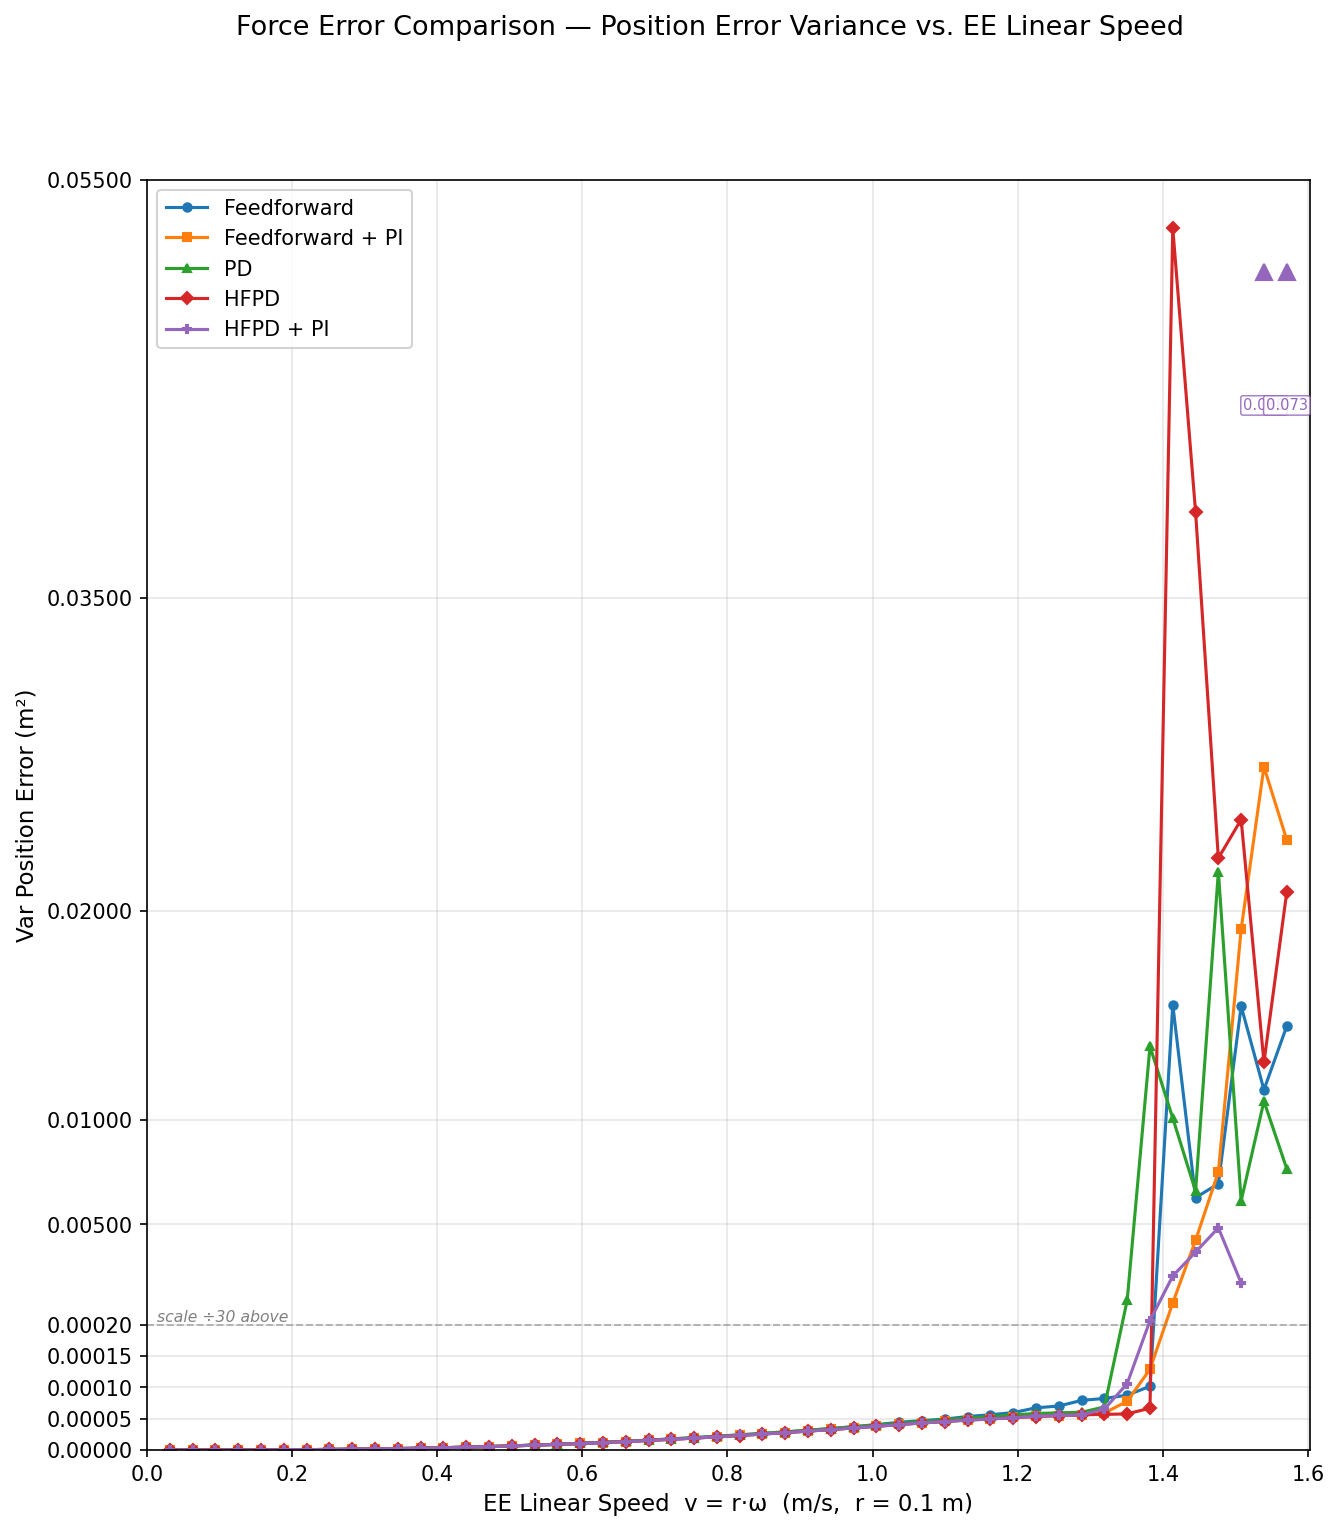
\includegraphics[width=\textwidth]{images/position_var_comparison.png}
        \caption{}
        \label{fig:position_var_comparison}
    \end{subfigure}
    \caption{position error comparison}
    \label{fig:speed_sweep_position_error}
\end{figure}
Position error remains uniformly small for all methods at speeds below a critical
threshold, in the range of $3$--$14\,\mathrm{mm}$.
Figure ~\ref{fig:position_error_comparison} shows a sharp, abrupt increase in $\bar{e}_p$ is observed for all methods near
$v \approx 1.38$--$1.41\,\mathrm{m/s}$, indicating loss of trajectory tracking.
The PD controller degrades first, with $\bar{e}_p$ jumping from
$0.018\,\mathrm{m}$ to $0.112\,\mathrm{m}$ at $v = 1.38\,\mathrm{m/s}$
($\omega \approx 13.8\,\mathrm{rad/s}$).
The HFPD\,+\,PI and feedforward\,+\,PI methods degrade more gradually at
$v = 1.41\,\mathrm{m/s}$ ($\bar{e}_p = 0.057\,\mathrm{m}$ and
$0.023\,\mathrm{m}$, respectively), suggesting that integral force correction
moderates the destabilising effect of high-frequency contact dynamics.
Above $v \approx 1.5\,\mathrm{m/s}$ all methods diverge, exhibiting catastrophic instability.

\subsection{Detailed Analysis at Representative Speeds}
We now examine the force and motion tracking behavior at representative 
end-effector speeds. For each selected end effector speed, the force tracking 
error is defined as $e_F = F_z - F_d$ and reported with sign. A positive error indicates loss of contact or insufficient force application; 
for example, when the end-effector loses contact entirely, $F_z = 0\,\mathrm{N}$ 
and the error reaches $e_F = 0 - (-8) = +8\,\mathrm{N}$. Conversely, a negative 
error indicates excessive force against the surface; for example, $F_z = -10\,\mathrm{N}$ 
yields $e_F = -10 - (-8) = -2\,\mathrm{N}$.
\begin{figure}[htbp]
    \centering
    % Row 1
    \begin{subfigure}[b]{0.9\textwidth}
        
\includegraphics[width=\textwidth]{images/speed_3.4/force_tracking.png}
        \caption{signed force error $e_F = F_z - F_d$ for all controllers}
        \label{fig:speed_3.4/force_tracking}
    \end{subfigure}

    \vspace{0.5em}  % vertical gap between rows

    % Row 2
    
    \begin{subfigure}[b]{0.9\textwidth}
        
\includegraphics[width=\textwidth]{images/speed_3.4/position_tracking_xyz.png}
        \caption{end-effector position tracking in $x$, $y$, $z$}
        \label{fig:speed_3.4/position_tracking}
    \end{subfigure}

    \caption{Force tracking error and end-effector trajectory at 
$v \approx 1.07\,\mathrm{m/s}$ ($\omega = 3.4\pi\,\mathrm{rad/s}$)}
    \label{fig:force_position_details_3.4}
\end{figure}

Figure~\ref{fig:speed_3.4/position_tracking} presents the position tracking 
performance at $v = 1.068\,\mathrm{m/s}$ ($\omega \approx 3.4\pi\,\mathrm{rad/s}$). All controllers maintain accurate trajectory following throughout the 
motion. A transient deviation is observed during the first $0.5\,\mathrm{s}$, 
attributable to the approach phase prior to surface contact, after which all 
methods converge to the desired trajectory.

The corresponding force tracking results, shown in 
Figure~\ref{fig:speed_3.4/force_tracking}, reveal significant differences among the controllers 
at this speed. The pure feedforward ($F_\text{des}$) controller fails to maintain 
stable contact, exhibiting force errors up to $8\,\mathrm{N}$, which means complete loss of contact. The PD controller, or down to $-20\,\mathrm{N}$, which means
excessive surface penetration. The PD controller
displays a notably wide error band, indicating high-frequency force oscillations 
at this end-effector speed. Both the PD controller and the feedforward with PI 
($F_\text{des}$ + PI) exhibit a mean force error exceeding $1.5\,\mathrm{N}$ and 
peak errors of approximately $4\,\mathrm{N}$.

In contrast, HFPD controller and its PI-augmented variant 
(HFPD + PI) achieve substantially reduced force tracking errors. In particular, 
HFPD + PI attains a mean force error of $0.235\,\mathrm{N}$ and a maximum force 
error of $0.524\,\mathrm{N}$, demonstrating (to be filled).

\begin{figure}[htbp]
    \centering
    % Row 1
    \begin{subfigure}[b]{0.9\textwidth}
        
\includegraphics[width=\textwidth]{images/speed_3.8/force_tracking.png}
        \caption{signed force error $e_F = F_z - F_d$ for all controllers}
        \label{fig:speed_3.8/force_tracking}
    \end{subfigure}

    \vspace{0.5em}  % vertical gap between rows

    % Row 2

    \begin{subfigure}[b]{0.9\textwidth}
        
\includegraphics[width=\textwidth]{images/speed_3.8/position_tracking_xyz.png}
        \caption{end-effector position tracking in $x$, $y$, $z$}
        \label{fig:speed_3.8/position_tracking}
    \end{subfigure}

    \caption{Force tracking error and end-effector trajectory at 
$v \approx 1.10\,\mathrm{m/s}$ ($\omega = 3.8\pi\,\mathrm{rad/s}$)}
    \label{fig:force_position_details_3.8}
\end{figure}

Based on the speed sweep results, three distinct operating regimes are identified 
for the HFPD and HFPD+PI controllers within the circular drawing scenario at 
radius $r = 0.1\,\mathrm{m}$. Below $v \approx 1.07\,\mathrm{m/s}$ 
($\omega \approx 3.4\pi\,\mathrm{rad/s}$), both controllers maintain stable 
contact and accurate force tracking without loss of contact or excessive surface 
penetration. In the intermediate regime, 
$1.07 \lesssim v \lesssim 1.38\,\mathrm{m/s}$ 
($3.4\pi \lesssim \omega \lesssim 4.4\pi\,\mathrm{rad/s}$), intermittent loss 
of contact occurs; however, the controllers recover without producing dangerous 
penetration forces, as illustrated in Figure~\ref{fig:force_position_details_3.8}. 
Beyond $v \approx 1.38\,\mathrm{m/s}$ ($\omega \approx 4.4\pi\,\mathrm{rad/s}$), 
force tracking degrades irrecoverably for all evaluated methods and precise 
trajectory following can no longer be maintained, as shown in 
Figure~\ref{fig:force_position_details_4.4}.

In summary, HFPD and HFPD+PI provide consistently superior force tracking 
relative to all other evaluated controllers across the full stable operating 
range, with HFPD+PI achieving the lowest steady-state force error at every speed within operational range.

\begin{figure}[htbp]
    \centering
    % Row 1
    \begin{subfigure}[b]{0.9\textwidth}
        
\includegraphics[width=\textwidth]{images/speed_4.4/force_tracking.png}
        \caption{signed force error $e_F = F_z - F_d$ for all controllers}
        \label{fig:speed_4.4/force_tracking}
    \end{subfigure}

    \vspace{0.5em}  % vertical gap between rows

    % Row 2

    \begin{subfigure}[b]{0.9\textwidth}
        
\includegraphics[width=\textwidth]{images/speed_4.4/position_tracking_xyz.png}
        \caption{end-effector position tracking in $x$, $y$, $z$}
        \label{fig:speed_4.4/position_tracking}
    \end{subfigure}

    \caption{Force tracking error and end-effector trajectory at 
$v \approx 1.38\,\mathrm{m/s}$ ($\omega = 4.4\pi\,\mathrm{rad/s}$)}
    \label{fig:force_position_details_4.4}
\end{figure}







\section{Simulation: Flat Surface — With Surface Friction}

% TODO (FILL): Show how friction degrades force tracking. Explain the role
% of tangential friction force in the constraint subspace and how it differs
% from simple stiction.

\begin{figure}[htbp]
    \centering
    % TODO (PLOT): Force tracking comparison: Bruno+velocity_term with no
    % friction vs. low friction vs. full friction.
    \missingfigure{Force tracking: no friction vs.\ low friction vs.\ full friction}
    \caption{Force tracking comparison for the Bruno\,+\,velocity-term method
             under no friction, low friction, and full friction conditions.}
    \label{fig:friction_comparison}
\end{figure}

\begin{figure}[htbp]
    \centering
    % TODO (PLOT): Friction norm over time — non-constant tangential force
    % but relatively stable z-component.
    \missingfigure{Friction norm over time}
    \caption{Friction norm over time showing the non-constant tangential
             force component and the relatively stable $z$-component.}
    \label{fig:friction_norm}
\end{figure}

% TODO (FILL): angular speed sweep across 5 methods. Explain why faster motion
% increases force coupling and why the velocity-term compensation becomes
% more critical.


\section{Contact Force Compensation Analysis}

% TODO (FILL): Deep dive into contact_force_compensation = Λ_φ J_φ M⁻¹ Jᵀ_motion F_ext_x.
% Show its effect when added (+1), subtracted (–1), or zeroed.
% Conclusion: compensation term destabilises with full friction.

\begin{figure}[htbp]
    \centering
    % TODO (PLOT): Component visualisation: control_force_compensation,
    % contact_force_compensation, velocity_term over time in force subspace.
    \missingfigure{Compensation components over time in the force subspace}
    \caption{Component visualisation of \texttt{control\_force\_compensation},
             \texttt{contact\_force\_compensation}, and \texttt{velocity\_term}
             over time in the force subspace.}
    \label{fig:compensation_components}
\end{figure}


\section{Impedance Gain Sensitivity}

% TODO (FILL): Show how impedance_pos values (100, 500, 1000, 1500) affect
% EE stability and force tracking. Identify stable operating range.

\begin{figure}[htbp]
    \centering
    % TODO (PLOT): Force tracking and EE position for impedance_pos ∈
    % {500, 1000, 1500} — 3-subplot comparison.
    \missingfigure{Force tracking and EE position for impedance\_pos $\in\{500, 1000, 1500\}$}
    \caption{Force tracking and end-effector position for
             $k_\text{imp} \in \{500, 1000, 1500\}$\,N/m --- three-subplot
             comparison.}
    \label{fig:impedance_sensitivity}
\end{figure}


% ==================================================================
\chapter{Simulation Experiments --- Slope Surface (\texorpdfstring{$30^\circ$}{30 deg})}
% ==================================================================

\section{Slope Setup and Constraint Frame Adaptation}

% TODO (FILL): Describe MuJoCo XML modification for 30° slope, coordinate
% frame rotation, and how J_φ is computed using the rotated S_f. Explain
% why J̇_φ ≈ 0 for planar slope.

\begin{figure}[htbp]
    \centering
    % TODO (PLOT): MuJoCo scene: Panda on slope environment with constraint
    % frame axes overlaid.
    \missingfigure{MuJoCo scene: Panda on slope with constraint frame axes}
    \caption{MuJoCo simulation scene of the Panda robot on the $30^\circ$
             slope environment with the constraint frame axes overlaid.}
    \label{fig:mujoco_slope}
\end{figure}


\section{Velocity Term Analysis on Slope}

% TODO (FILL): Show J̇_φ computation problem (was zero due to un-updated
% Pinocchio data). After fix, analyse two sub-terms:
% Λ_φ J_φ M⁻¹ C q̇ (red) and –Λ_φ J̇_φ q̇ (blue). Show they nearly cancel.

\begin{figure}[htbp]
    \centering
    % TODO (PLOT): Velocity term components (red: Coriolis part,
    % blue: J̇_φ part) and their sum ≈ 0 on slope.
    \missingfigure{Velocity term components on slope: Coriolis (red) and $\dot{J}_\Phi$ (blue)}
    \caption{Velocity term components on the slope: Coriolis part (red) and
             $-\Lambda_\Phi \dot{J}_\Phi \dot{q}$ part (blue), and
             their sum which is approximately zero.}
    \label{fig:velocity_term_slope}
\end{figure}

\begin{figure}[htbp]
    \centering
    % TODO (PLOT): Force tracking: with J̇_φ (Pinocchio attachment frame)
    % vs. without J̇_φ — showing negligible difference on slope.
    \missingfigure{Force tracking: with $\dot{J}_\Phi$ vs.\ without $\dot{J}_\Phi$ on slope}
    \caption{Force tracking on the slope with and without the
             $\dot{J}_\Phi$ term, demonstrating the negligible difference.}
    \label{fig:slope_jdot_comparison}
\end{figure}


\section{Slope Performance: Slow vs.\ Fast}

% TODO (FILL): Present force tracking at π/4 and π rad/s on 30° slope.
% Compare with flat surface results. Note that Bruno+velocity_term performs
% well in frictionless environment.

\begin{figure}[htbp]
    \centering
    % TODO (PLOT): Contact force tracking on slope: π/4 rad/s (top) and
    % π rad/s (bottom) — desired vs. actual.
    \missingfigure{Contact force tracking on slope: $\pi/4$\,rad/s (top) and $\pi$\,rad/s (bottom)}
    \caption{Contact force tracking on the $30^\circ$ slope at
             $\pi/4$\,rad/s (top) and $\pi$\,rad/s (bottom), showing
             desired versus actual force.}
    \label{fig:force_slope}
\end{figure}

\begin{figure}[htbp]
    \centering
    % TODO (PLOT): EE trajectory on slope: 3D path plot and X/Y/Z time series.
    \missingfigure{End-effector trajectory on slope: 3D path and X/Y/Z time series}
    \caption{End-effector trajectory on the slope: three-dimensional path
             plot (left) and $X/Y/Z$ position time series (right).}
    \label{fig:ee_trajectory_slope}
\end{figure}


\section{Franka vs.\ KUKA Comparison in Simulation}

% TODO (FILL): Describe adaptation from KUKA iiwa to Franka Panda XML
% (torque actuator, attachment collision). Note Panda has larger force error
% and less stability at π rad/s compared to KUKA.

\begin{figure}[htbp]
    \centering
    % TODO (PLOT): Side-by-side force tracking: KUKA iiwa vs. Franka Panda,
    % with and without friction, at π rad/s.
    \missingfigure{Force tracking: KUKA iiwa vs.\ Franka Panda, with/without friction, $\pi$\,rad/s}
    \caption{Side-by-side force tracking comparison between the KUKA iiwa
             and Franka Panda at $\pi$\,rad/s, with and without friction.}
    \label{fig:kuka_vs_panda}
\end{figure}


% ==================================================================
\chapter{Real Robot Experiments}
% ==================================================================

\section{Hardware and Software Setup}

% TODO (FILL): Describe Franka Panda hardware, libfranka interface,
% pylibfranka Python wrapper, Pinocchio for real-time dynamics,
% communication constraints (1 kHz loop, profiling to meet deadline).
% Mention Docker container setup.

\begin{figure}[htbp]
    \centering
    % TODO (PLOT): Photo of real Franka Panda robot setup in the lab with
    % slope/surface fixture.
    \missingfigure{Photo: real Franka Panda robot setup in the lab}
    \caption{The real Franka Panda robot setup in the laboratory with the
             slope/surface fixture.}
    \label{fig:real_panda}
\end{figure}


\section{Unified Simulation-to-Real Interface}

% TODO (FILL): Explain the MuJoCo/libfranka API unification (wrapping MuJoCo
% with libfranka interface, removing dof_ids dependency). Describe the
% two-phase controller: approach (CartesianPD) → hybrid control.

\begin{figure}[htbp]
    \centering
    % TODO (PLOT): Software architecture diagram: unified controller class
    % with MuJoCo and libfranka backends.
    \missingfigure{Software architecture: unified controller with MuJoCo and libfranka backends}
    \caption{Software architecture diagram showing the unified controller
             class with MuJoCo and libfranka backends.}
    \label{fig:software_architecture}
\end{figure}


\section{Real Robot Results: Flat Surface}

% TODO (FILL): Present force tracking results on physical robot. F_ext
% estimated from joint torque observer (no F/T sensor). Compare with sim.

\begin{figure}[htbp]
    \centering
    % TODO (PLOT): Real robot: contact force z (desired vs. measured) over
    % time during circle drawing.
    \missingfigure{Real robot: contact force $z$ over time during circle drawing}
    \caption{Real-robot contact force ($z$-direction) over time during circle
             drawing on the flat surface, showing desired versus measured
             force.}
    \label{fig:real_force_flat}
\end{figure}

\begin{figure}[htbp]
    \centering
    % TODO (PLOT): Real robot: joint torques during approach and hybrid
    % control phases.
    \missingfigure{Real robot: joint torques during approach and hybrid control}
    \caption{Real-robot joint torques during the approach phase and the
             hybrid control phase.}
    \label{fig:real_torques}
\end{figure}

\begin{figure}[htbp]
    \centering
    % TODO (PLOT): Real robot: EE position tracking X/Y/Z vs. time.
    \missingfigure{Real robot: end-effector position tracking X/Y/Z}
    \caption{Real-robot end-effector position tracking ($X/Y/Z$ versus time).}
    \label{fig:real_ee_position}
\end{figure}


\section{Real Robot Results: Slope Surface}

% TODO (FILL): Results for slope experiment on real robot. Discuss
% discrepancies from simulation (real friction, model mismatch, flexibility).

\begin{figure}[htbp]
    \centering
    % TODO (PLOT): Real robot on slope: contact force tracking comparison
    % vs. simulation.
    \missingfigure{Real robot on slope: contact force vs.\ simulation}
    \caption{Real-robot contact force tracking on the slope surface compared
             with the simulation results.}
    \label{fig:real_force_slope}
\end{figure}


\section{Discussion: Sim-to-Real Gap}

% TODO (FILL): Analyse sources of difference: joint flexibility, unmodelled
% friction, contact model (MuJoCo soft contact vs. real hard contact),
% communication latency. Force feedback from external torque observer is
% less accurate than F/T sensor.


% ==================================================================
\chapter{Discussion}
% ==================================================================

\section{Comparison of Force Control Strategies}

% TODO (FILL): Structured comparison: F_desired, PD, PI, Bruno+velocity_term.
% When does each method shine/fail?

\begin{figure}[htbp]
    \centering
    % TODO (PLOT): Summary comparison: force tracking error, stability,
    % robustness to friction, sim-to-real transferability — table or radar
    % chart across 4 methods.
    \missingfigure{Summary comparison of four force control methods}
    \caption{Summary comparison of force tracking error, stability, robustness
             to friction, and sim-to-real transferability across the four
             control methods.}
    \label{fig:method_comparison}
\end{figure}


\section{Role of Friction}

% TODO (FILL): Friction is the dominant disturbance. In frictionless
% environments Bruno+velocity_term achieves near-perfect tracking. With
% friction, contact_force_compensation becomes destabilising. The velocity
% term compensates Coriolis but cancels with J̇_φ on slope.


\section{Flat vs.\ Slope Generalisation}

% TODO (FILL): The framework generalises naturally via the constraint-frame
% rotation. Key insight: J̇_φ ≈ 0 for planar surfaces simplifies velocity
% compensation significantly.


\section{Limitations}

The following limitations were identified during the course of this work:

\begin{itemize}
    \item No force/torque sensor was available; contact force is estimated
          from a joint torque observer, which is less accurate especially
          in the presence of friction.
    \item Only planar surfaces were tested; curved surfaces (e.g.\ a sphere)
          would require a time-varying selection matrix $S_f$.
    \item High-speed motions at $\pi$\,rad/s produce stability challenges on
          the Panda due to its inertia and joint flexibility.
    \item Null-space control has a marginal effect on contact force.
\end{itemize}


% ==================================================================
\chapter{Conclusion and Future Work}
% ==================================================================

\section{Conclusion}

% TODO (FILL): Summarise: successfully implemented hybrid force-impedance
% control on Franka Panda in simulation and reality. Bruno velocity-term
% method achieves best force tracking in frictionless conditions. Slope
% extension validated. Real-robot transfer demonstrated.


\section{Future Work}

Promising directions for future work include:

\begin{itemize}
    \item Extending the framework to curved surfaces (cylinder, sphere) where
          $\dot{J}_\Phi \neq 0$ and $S_f$ is time-varying.
    \item Incorporating an external force/torque sensor for more accurate
          force feedback.
    \item Developing a friction compensation module using the adaptive friction
          estimator of~\citeauthor{huang2025}~\cite{huang2025}.
    \item Applying the controller to real contact tasks such as polishing,
          wiping, or ultrasound scanning.
    \item Investigating energy-tank-based passivity guarantees for high-speed
          operation.
\end{itemize}


% ==================================================================
\appendix
% ==================================================================

\chapter{Mathematical Derivations}

% TODO (FILL): Full derivation of the hybrid force-impedance equations
% following the paper digest notes: eq. 7→8→9→10, 10+12+1→11, 8→13,
% 1+13→14, 15→17, 14+18+15→19.

\begin{figure}[htbp]
    \centering
    % TODO (PLOT): Equation derivation tree / step-by-step proof diagram.
    \missingfigure{Equation derivation tree for the hybrid force-impedance equations}
    \caption{Step-by-step derivation tree for the hybrid force-impedance
             control equations.}
    \label{fig:derivation_tree}
\end{figure}


\chapter{Controller Parameters}

% TODO (FILL): Table of all control gains used in simulation and real-robot
% experiments: Kp, Kd (motion), Kp_force, Kd_force, Ki (force),
% impedance_pos, impedance_ori, friction parameters.


\chapter{MuJoCo XML Configuration}

% TODO (FILL): Key XML snippets for slope geom, Panda actuator configuration
% (motor/torque), contact condim and friction settings.


\chapter{Additional Experimental Plots}

\begin{figure}[htbp]
    \centering
    % TODO (PLOT): Additional force tracking plots for PD controller with
    % different Kp/Kd values (π/4 and π speeds).
    \missingfigure{Force tracking: PD controller with different Kp/Kd values}
    \caption{Additional force tracking plots for the PD controller with
             varying $K_p$/$K_d$ values at $\pi/4$\,rad/s and
             $\pi$\,rad/s.}
    \label{fig:pd_gains_sweep}
\end{figure}

\begin{figure}[htbp]
    \centering
    % TODO (PLOT): Friction norm over time on flat surface under different
    % condim settings.
    \missingfigure{Friction norm over time under different condim settings}
    \caption{Friction norm over time on the flat surface under different
             MuJoCo \texttt{condim} settings.}
    \label{fig:friction_condim}
\end{figure}

\begin{figure}[htbp]
    \centering
    % TODO (PLOT): q0 drift analysis: joint reference tracking with fixed
    % vs. IK-computed reference.
    \missingfigure{$q_0$ drift analysis: fixed vs.\ IK-computed reference}
    \caption{$q_0$ drift analysis comparing joint reference tracking with a
             fixed reference versus an IK-computed reference.}
    \label{fig:q0_drift}
\end{figure}


% ==================================================================
% References — paste \printbibliography from main.tex here, or leave
% \printbibliography in its original location and add your .bib entries
% to DEMO-TUDaBibliography.bib. Example BibTeX keys used above:
%
%   iskandar2023   → Iskandar et al. (2023)
%   dietrich2021   → Dietrich et al. (2021)
%   khatib1987     → Khatib (1987)
%   raibertcraig1981 → Raibert & Craig (1981)
%   chiacchio1991  → Chiacchio et al. (1991)
%   huang2025      → Huang et al. (2025)
%   hogan1985      → Hogan (1985)
% ==================================================================

\chapter{Verwendung}
Die Klasse kann wie für Dokumentenklassen üblich eingebunden werden
\begin{verbatim}
\documentclass[thesis]{tudapub}
\end{verbatim}
Die Option \code{thesis} wechselt hierbei in den Modus, der spezielle Features für Abschlussarbeiten freischaltet, die in diesem Dokument beschrieben werden.

Darüber hinaus lässt sich die Klasse verwenden wie die Standard-KOMA-Script-Klasse, auf der sie basiert.
Voreingestellt ist hierbei \code{scrreprt}.

Allgemein bietet \KOMAScript{} viele Möglichkeiten zu Anpassungen. Wie in der tudapub-Demo-Datei beschrieben, können hier jedoch nicht alle erläutert werden, ein Blick in die offizielle Dokumentation ist daher häufig hilfreich \cite{scrguide}.

\section{Sprachanpassung}
Der Modus für Abschlussarbeiten setzt einige sprachabhängige Bezeichnungen.
Teilweise ist Deutsch für diese Elemente als Hauptsprache vorgeschrieben (z.\,B. die Selbstständigkeitserklärung). Für die korrekte Verarbeitung wird daher ein Paket zur Sprachanpassung benötigt.
TUDa-CI verwendet hierfür das babel-Paket.

Dies wird jedoch nicht automatisch geladen, da hierfür die Konfiguration der Sprachen bekannt sein müsste. Die Demo-Dateien für Abschlussarbeiten (\file{DEMO-TUDaThesis.tex}/""\file{DEMO-TUDaPhD.tex}) laden hierfür die Konfiguration:
\begin{verbatim}
    \usepackage[english, main=german]{babel}
\end{verbatim}
Diese ist für ein Dokument mit Deutsch als Hauptsprache und Englischen Elementen.
Die Hauptsprache wird als Wert der Option \verb+main=+ übergeben.
Das Laden von \verb+german+ wird in den Fällen, in denen es von TUDa-CI benötigt wird, automatisch ausgelöst.
Für eine bessere Übersichtlichkeit ist es dennoch hilfreich es dort aufzuführen.

Falls die Hauptsprache nicht Deutsch ist, wäre daher die folgende Konfiguration sinnvoll:
\begin{verbatim}
    \usepackage[german, main=<Hauptsprache>]{babel}
\end{verbatim}

\section{Übergabe der Titeldaten}

Die Daten werden analog zur klassischen Titeleierzeugung mit \verb+\maketitle+ übergeben. Allerdings wurden die Felder um ein paar speziellere Daten erweitert. Sofern nicht anders angegeben, verfügen alle Makros über ein notwendiges Argument für die Datenübergabe, z.\,B.
\begin{verbatim}
    \title{\LaTeX{} im Corporate Design der TU Darmstadt}
\end{verbatim}
Es ist zu beachten, dass für die Erzeugung der Titelseite nach Übergabe aller Daten \verb+\maketitle+ aufgerufen werden muss.

Falls eine Layoutanpassung der Titelseite notwendig ist, gelten die in der TUDa-CI-Dokumentation \cite{tuda-ci}  geschilderten Optionen. Dort finden sich auch Hinweise zur Platzierung von Sponsorenlogos.

\begin{description}\setkomafont{descriptionlabel}{\ttfamily\textbackslash}
	\item[title] Titel, wird in sehr großer Schrift im obersten Block der Titelseite platziert. Die Schriftgröße ist aufgrund der Häufigkeit für lange Titel kleiner gewählt als für andere Publikationen.
	\item[subtitle] Untertitel. Dieses Feld kann alternativ für eine Übersetzung genutzt werden.
	\item[author] Der Autor/dir Autoren. Mehere Autoren werden durch \verb+\and+ getrennt.
	\item[studentID] Matrikelnummer. Nach den Vorgaben des Templates ist diese Angabe immer optional.
	\item[birthplace] Geburtsort.
	\item[reviewer] Gutachter. Mehrere Gutachter werden, wie Autoren durch \verb+\and+ getrennt. Die Nummerierung läuft von links nach rechts.
	      \minisec{Änderung des Bezeichners}
	      Die Änderung des Bezeichners ist über ein optionales Argument möglich:
\begin{verbatim}
        \reviewer[Ersatzbezeichner]{Name1 \and Name2}
\end{verbatim}
	      Um die numerische Benennung abzuändern ist es zusätzlich möglich statt dem Ersatzbezeichner eine Kommaliste zu übergeben:
\begin{verbatim}
        \reviewer*[Bezeichner1, Bezeichner2]{Name1 \and Name2}
\end{verbatim}
	      In diesem Fall entfällt die Nummerierung vor dem Bezeichner. Soll z.\,B. den Formulierungen der Promotionsordnung entsprochen werden, gilt:
\begin{verbatim}
        \reviewer[Erstreferent\_in,Koreferent\_in]{Name1 \and Name2}
\end{verbatim}
	      Für die Erstellung Fachbereichsspezifischer Templates existiert hierfür auch ein Makro, dass ohne den Aufruf von \verb+\reviewer+ Änderungen zulässt.
\begin{verbatim}
        \setupReviewName{Ersatzwort für „Gutachten“}
\end{verbatim}
	      Setzt die ersten beiden Bezeichner. Alternativ ist es auch möglich Positionen einzeln zu benennen \verb+\setupReviewName[1]{Erstferent}+, eine Übergabe als Komma-Liste ist als \verb+\setupReviewName*{Bezeicher1,Bezeicher2}+ möglich.

	      Ab Version 3.26 werden die Gutachter nicht mehr auf der Titelrückseite genannt. Dies wird über die \verb+thesis+ Option \verb+reviewer-on-uppertitleback+ gesteuert. Voreingestellt ist der Wert \verb+false+.
	\item[institution] Einrichtung. Dieser Eintrag, wie auch die beiden folgenden, werden unterhalb des Logos auf der Titelseite platziert.
	\item[department] Fach-/Studienbereich, allerdings ist die oben genannte Option zu bevorzugen. Die Verarbeitung des Arguments erfolgt jedoch analog.

	      Dieses Makro verfügt jedoch zusätzlich über die Möglichkeit abweichende Einträge gegenüber den Vorgaben anzugeben. Insbesondere wenn eine gesonderte Formulierung gegenüber der voreingestellten \enquote{im Fachbereich} und ihren Varianten notwendig ist. Hierfür liefert \code{\textbackslash{}department} ein optionales Argument:

\begin{verbatim}
    \department[Ersatztext]{Kürzel/Bezeichnung}
\end{verbatim}
	      Zusätzlich gibt es ab Version 2.01 auch die Möglichkeit den gesamten Text \enquote{im Fachbereich <Bereichsbezeichnung>}, sowie die Angabe in der Infobox auf der Titelseite zu ersetzen. Dies geschieht über die gesternte Variante:
\begin{verbatim}
    \department*[Text für die Box]{Text zwischen Typ und Autor}
\end{verbatim}
	\item[group] Arbeitsgruppe.
	\item[submissiondate] Datum der Einreichung
	\item[examdate] Datum der Disputation
	\item[date] Beliebiges Datum. Wird über \verb|datename| bezeichnet.
	\item[publishers] Wird hier für die Ortsangabe verwendet und ist mit \enquote{Darmstadt}, bzw. \enquote{Darmstadt, Technische Universität Darmstadt} (bei Dissertationen) vorbelegt.
	\item[tuprints] \label{page:tuprints}Übergabe der Daten, sofern das Dokument über TUprints Veröffentlicht werden soll.
\begin{verbatim}
    \tuprints{
        printid=12345,
        urn=123456,
        year=2022
    }
\end{verbatim}
	      Falls das Argument kein Gleichheitszeichen erkennt, wird der Wert als \code{printid} gesetzt und keine URN angegeben.

	      Die printid is die ID-Nummer des TUprints-Eintrags. Die urn ist ein dauerhaft eindeutig zitierfähiger Bezeichner für das Dokument. Die Nummer entspricht bei TUprints der printid mit Ergänzung einer Prüfziffer. Beide Angaben sind in den Details des TUprints-Eintrags zu finden.

	      \minisec{Lizenzangabe}
	      Ab Version 2.07 ist es zudem möglich einen eigenen Lizenztext über den Schlüssel \verb|license=<Text>| zu übergeben. Dieser ersetzt dann die voreingestellte Lizenzangabe.

	      Es existieren (seit v3.08) vorgefertigte Werte für die Option \verb|license|, um eine einfachere Anpassung zu ermöglichen. Diese lauten:

	      \parbox[t]{.5\linewidth}{%
		      \ttfamily
		      \href{https://creativecommons.org/licenses/by/4.0/}{cc-by-4.0} \textnormal{Voreinstellung seit Version 4.0}\par
		      \href{https://creativecommons.org/licenses/by-sa/4.0/}{cc-by-sa-4.0}\par
		      \href{https://creativecommons.org/licenses/by-nc-sa/4.0/}{cc-by-nc-sa-4.0}\par
		      \href{https://creativecommons.org/licenses/by-nc-/4.0/}{cc-by-nc-4.0}\par
	      }%
	      \parbox[t]{.5\linewidth}{
		      \ttfamily
		      \href{https://creativecommons.org/licenses/by-nd/4.0/}{cc-by-nd-4.0}\par
		      \href{https://creativecommons.org/licenses/by-nc-nd/4.0/}{cc-by-nc-nd-4.0}\par
		      \href{https://rightsstatements.org/page/InC/1.0/}{inc-1.0}\textnormal{ (Ab Version 3.36)}
		      \href{https://creativecommons.org/licenses/by-nc-nd/2.0/}{cc-by-nc-nd-2.0-de}\par
	      }

	      Die Einführung dieser Option war Bestandteil der Vorbereitung zur Anpassung der Standardlizenz.
	      Die entsprechende Diskussion findet sich unter \url{https://github.com/tudace/tuda_latex_templates/issues/251}. Die Anpassung der Voreinstellung bei TUDa-CI geschah mit Version 4.0.

	      Unterstützung bei der Wahl einer passenden Creative Commons Lizenz bietet die ULB der TUDa unter https://www.ulb.tu-darmstadt.de/dpub  oder  das CC-Projekt sebst über seinen Lizenzfinder unter \url{http://creativecommons.org/choose/}.
	      Die TU Darmstadt empfiehlt in Ihrer Publikationsrichtlinie und Open-Access-Policy die Nutzung der offenen CC BY 4.0 Lizenz.

	      Falls ein von den oben gelisteten Schlüsseln abweichender Wert gesetzt wird, wird ebendieser direkt an der Stelle des Lizenztextes verwendet. Sofern der Text Gleichheitszeichen oder Kommata enthält ist eine Gruppierung notwendig.
	\item[titlegraphic] Hier kann Code übergeben werden, der den farbigen Block im unteren Teil der Titelseite ersetzt. Details sind in der allgemeinen TUDaPub-Dokumentation beschrieben \cite{tuda-ci}.
	\item[titleintro] Ab Version 2.03 kann zusätzlich über diesen Hook ein beliebiger Text direkt nach dem Untertitel und vor den automatischen Daten ergänzt werden.
	\item[titleaddendum] Wie \code{\tbs{}titleintro} jedoch als letztes Element des Blocks.
\end{description}

\section{Weitere Makros}
Das Makro \verb+\affidavit+ erzeugt eine Selbstständigkeitserklärung mit Unterschriftenzeile. Hier wird der oben übergebene Name/Signatur eingefügt.
In diesem Dokument findet sich das Affidavit direkt nach der Titelei.

Ab Version 3.32 entfällt die seit Version 3.06 unterstütze Unterscheidung zwischen einem Affidavit für digitale oder gedruckte Abgaben. Aus Kompatibilitätsgründen werden die Optionen weiterhin verstanden, allerdings bewirken nun beide das gleiche. Der Text entstammt von  \url{https://www.tu-darmstadt.de/studieren/studierende_tu/studienorganisation_und_tucan/hilfe_und_faq/artikel_details_de_en_37824.de.jsp} (Stand 2023-06-19). Es ist zwingend erforderlich, dass Studierende vor der Abgabe einer Arbeit überprüfen, ob der Text der geforderten Fassung entspricht.

Dissertationen verwenden hier einen anderen Text, für die Unterscheidung wird die Affidavit-Option \verb+affidavit=dr+ intern verwendet.

Version 3.20 ermöglicht zusätzlich die Übergabe weiterer Optionen für den Signatur-Namen, ein Signatur-Bild oder die Ortsangabe.
Inwieweit diese Optionen verwendet werden dürfen ist jeweils vor der Verwendung durch die Nutzer:in abzuklären.
TUDa-CI kann hierfür keine gesicherte Aussage treffen.
\begin{verbatim}
    \affidavit[
        signature=Signaturname,
        signature-image={\includegraphics[width=\width]{signaturbild}}
    ]
\end{verbatim}
Eine vertikale Verschiebung des Signaturbildes ist nicht direkt implementiert, ist jedoch mit der Verwendung des \LaTeX-Makros \verb+\raisebox{<Verschiebung>}{<Inhalt>}+ problemlos möglich.

Es besteht zusätzlich die Möglichkeit ein anderssprachiges Affidavit als Ergänzung mit abzudrucken. Um die Struktur und die ggf. notwendige Sprachumschaltung zu erledigen, existiert hierfür ab Version 2.03 eine Umgebung:

\begin{verbatim}
    \begin{affidavit*}[Babel-Sprachoption]{Überschrift}
        Text
    \end{affidavit*}
\end{verbatim}

Diese Variante verfügt bewusst über keine Unterschriftenzeile, da diese Version laut Verständnis der Entwickler keine rechtliche Verbindlichkeit besitzt.

Die Umgebung kann jedoch auch für besondere Formen der Erklärung genutzt werden. In diesem Fall kann eine zusätzliche Signaturzeile über
\begin{verbatim}
    \AffidavitSignature[Stadt]
\end{verbatim}
hinzugefügt werden. Die Vorbelegung für Stadt ist hierbei \enquote{Darmstadt}.
Ab Version 3.20 ist die Übergabe einer zusätzlichen Option für den Ort der Signatur auch als Option möglich.

\begin{verbatim}
    \affidavit[signature-location=Stadt]
\end{verbatim}

\section{Layout-Optionen mit Verstoß gegen das Corporate Design}

Die Zeilenlängen sind laut Corporate Design aus typografischer Sicht zu lang.
Daher existiert die Klassenoption \code{custommargins}, die für dieses Dokument aktiviert wurde (Wert \code{true}). Sie verfügt über die Werte \code{true}, \code{false} und \code{geometry} mit folgender Bedeutung:

\begin{description}
	\item[custommargins=false] Standardeinstellung von \cls{tudapub}. Die Ränder entsprechen den Vorgaben des Corporate Design Guidelines. Die Einstellung wird durch \pkg{geometry} durchgeführt. Eigene Anpassungen werden durch das Ausführen von \code{\textbackslash{}maketitle} überschrieben.
	\item[custommargins=true] Die Einstellungen des Corporate Design Guidelines werden nicht aktiviert. \pkg{geometry} wird nicht geladen. Dieser Modus entspricht der Standardeinstellung von \KOMAScript{}. Dadurch werden die Ränder nicht fest definiert, sondern auf Basis des \pkg{typearea}-Paketes berechnet \cite[vgl.][]{scrguide}.
	\item[custommargins=geometry]  Diese Variante wurde auf Wunsch zur Verfügung gestellt, allerdings wird darauf hingewiesen, dass manuelle Randeinstellungen oft nicht zu einem harmonischen Satzspiegel führt.
	      \pkg{geometry} wird, wie bei \code{false} geladen und vorkonfiguriert. Es ist allerdings möglich kleinere Anpassung durch die Verwendung des Makros \code{\textbackslash{}geometry} zu setzen. Die Einstellungen, die zu Beginn des Dokuments gelten werden gespeichert und nach der Titelseite wiederhergestellt.

	      Hierbei ist zu beachten, dass die Einstellungen als Ausgangspunkt den Voreingestellten Satzspiegel nutzen (je nach Option mit Randnotizspalte oder ohne). Es ist möglich diese Optionen vor den eigenen mit zurückzusetzen:
\begin{verbatim}
\geometry{
   reset,
   <Eigene Anpassungen>
}
\end{verbatim}
	      Die gilt insbesondere für die Optionen \code{includehead}, \code{includefoot}, \code{includemp}.
\end{description}

\minisec{Hinweis zu den Kopf-/Fußzeilen}
Wenn die Option \code{marginpar=true} gesetzt bleibt, ragen die Kopf- und Fußzeile über die Marginalspalte hinaus. Aus ästhetischen Gründen wird daher empfohlen in diesem Fall die Kopf- und Fußzeile  mit \code{marginpar=false}  auf den Textbereich zu beschränken.

Auch ist das Standard-Layout der Kolumnentitel wenig vorteilhaft, da die Kolumnentitel damit local größer sein können als die eigentliche Überschrift. (\code{headline=automark})
Deswegen kann über
\begin{verbatim}
\pagestyle{TUDa.headings}
\end{verbatim}
ein einfacherer Seitenstil ausgewählt werden, der die Nutzung mit lebenden Kolumnentitel erheblich vereinfacht. Dieser Stil ist über \pkg{scrlayer-scrpage} realisiert und kann entsprechend der \KOMAScript{}-Dokumentation angepasst werden.

\minisec{Hinweis zur Bindekorrektur}
Bei Verwendung einer Bindekorrektur (\code{BCOR=<Länge>}) wird diese nicht automatisch auch auf der Titelseite eingefügt. Für diesen Fall wurde mit Version 3.0 zusätzlich die Option \code{BCORtitlepage} hinzugefügt. Falls diese aktiviert wird, nimmt die Titelseite den Wert der Typearea Option \code{BCOR} auf der ersten Seite als Zusatz zum linken Rand hinzu.

\section{Spezielle Optionen für Abschlussarbeiten}
Die Klasse unterstützt alle Optionen der \file{tudapub}-Klasse. Darüber hinaus besteht über Wertzuweisung der Option \code{thesis} die Möglichkeit spezielle Einstellungen zu wählen.
Es ist prinzipiell möglich die Optionen auch direkt als Optionen zur \file{tudapub}-Klasse zu übergeben, allerdings ist dies aufgrund der schlechteren Übersicht nicht zu empfehlen.

Für dieses Dokument wurden beispielsweise die Optionen als
\begin{verbatim}
thesis={type=dr,dr=rernat}
\end{verbatim}
übergeben.

Im folgenden findet sich die Bedeutung der einzelnen Optionen:
\begin{description}
	\item[type=<Wert>] Auswahl des Typus. Dieser wird auf die Titelseite gesetzt und wählt zudem aus welche Daten für die Titelseite zwingend übergeben werden müssen.
	      Es stehen die folgenden Werte zur Verfügung (die Werte in Klammern sind die notwendigen Titeldaten):
	      \begin{itemize}
		      \item \code{sta}: Studienarbeit (title, author, date)
		      \item \code{diplom}: Diplomarbeit (title, author, submissiondate, reviewer, department)
		      \item \code{bachelor}: Bachelorarbeit (title, author, submissiondate, department, reviewer)
		      \item \code{master}: Masterarbeit (title, author, submissiondate, department, reviewer)
		      \item \code{pp}: Project-Proposal  (title, author, date, department)
		      \item \code{dr}: vorgelegte Dissertation (title, author, submissiondate, department, reviewer)
		      \item \code{drfinal}: genehmigte Dissertation (title, author, submissiondate, examdate, department, reviewer)
	      \end{itemize}
	      Wird ein Typus angegeben, der nicht erkannt wird, so wird der Text direkt übergeben. Notwendige Titelfelder über den Titel hinaus gibt es in diesem Fall nicht.
	\item[dr=<Kürzel>] Lädt einen der vordefinierten Texte für die Titelseite. Als Werte stehen bislang \code{rernat}, \code{rerpol}, \code{ing} und \code{phil} zur Verfügung. Zum Beispiel lädt der Wert \code{phil}:
	      \begin{quote}
		      Zur Erlangung des Grades eines Doktor der Philosophie (Dr.\,phil.)
	      \end{quote}
	      Sofern keiner dieser Werte dem angestrebten Titel entspricht, kann ein Text direkt übergeben werden.
\begin{verbatim}
    \drtext{Zur Erlangung des Grades \ldots}
\end{verbatim}
	\item[department=<Kürzel>] Die Fachbereiche sind fest als Textbausteine in Deutscher sowie Englischer Sprache hinterlegt. Diese Option ermöglicht die Auswahl als Dokumentenklassenoption. Aus Kompatibilitätsgründen kann jedoch auch das Makro \code{department}-Makro hierfür genutzt werden. Zur Verfügung stehen:\par
	      \begin{tabular}{@{}l@{${}\to{}$}l@{}}
		      arch  & Architektur\\
		      bauing& Bau- und Umweltingenieurwissenschaften\\
		      bio   &Biologie\\
		      chem  &Chemie\\
		      etit  &Elektrotechnik und Informationstechnik\\
		      gugw  &Gesellschafts- und Geschichtswissenschaften\\
		      humanw&Humanwissenschaften\\
		      inf   &Informatik\\
		      mb    &Maschinenbau\\
		      matgeo&Material- und Geowissenschaften\\
		      math  &Mathematik\\
		      phys  &Physik\\
		      wi    &Rechts- und Wirtschaftswissenschaften
	      \end{tabular}

	      Neben den Fachbereichen existieren für Abschlussarbeiten, die keine Dissertationen sind, auch Studienbereiche.
	      Falls das Kürzel nicht als Fachbereich hinterlegt ist, wird automatisch auf die Studienbereiche geprüft. Die Studienbereiche haben die folgenden Kürzel:

	      \begin{tabular}{@{}l@{${}\to{}$}l@{}}
		      ce&Computational Engineering\\
		      ese&Energy Science and Engineering\\
		      ist&Information Systems Engineering\\
		      mech&Mechanik\\
		      metro&Mechatronik
	      \end{tabular}

	      Falls etwas anderes als eines dieser Kürzel übergeben wird, wird der Text direkt verwendet und eine entsprechende Warnung ausgegeben.

	      Die Auswahl der Fachrichtung erzeugt zusätzlich eine Box auf der Titelseite unterhalb des Logos. Falls diese automatische Erstellung nicht gewünscht ist, kann dies über die Option \code{instbox=false} deaktiviert werden.
	\item[ignore-missing-data] Diese Option ist ein Schalter, der es ermöglicht die Fehlermeldung über nicht übergebene Titeldaten auszuschalten. In diesem Fall wird lediglich eine Warnung erzeugt, falls die angegeben Daten nicht mit den Anforderungen übereinstimmen.
\end{description}

\minisec{Abweichung von den Vorgaben für die Titelseite}
Da es möglich sein kann von dieser Vorgabe abzuweichen, existiert für Sonderfälle die Dokumentenklassenoption \code{instbox=false}. Damit wird die automatische Verarbeitung der Daten für die Boxen auf der der Titelseite unterdrückt. In diesem Fall ist der Autor jedoch selbst für die Einhaltung der Vorschriften verantwortlich. Weitere Information zur Konstruktion der Boxen findet sich in den Verwendungshinweisen der Basisklasse TUDaPub. Zusätzlich sei auf die Möglichkeiten des \code{\textbackslash{}department}-Makros verwiesen, sofern die Abweichung sich auf den Text beschränkt.

\section{Erhöhter Zeilenabstand -- Hinweise zum setspace-Paket}
Sofern die Vorgaben es erfordern, ist es möglich mit dem setspace-Paket den Durchschuss zu erhöhen. Allerdings beeinflusst dies natürlich sämtliche Zeilenabstände. Ein erhöhter Zeilenabstand sollte daher erst nach der Titelseite aktiviert werden. Allgemein ist es jedoch empfehlenswert auch für Verzeichnisse und sonstige Sonderelemente außerhalb des Fließtextes auf bei normalen Einstellungen zu bleiben.

Setspace liefert hierfür die Möglichkeit, das Paket ohne Optionen zu laden und später über Makros, wie \code{\tbs{}onehalfspacing} das Umschalten zu verzögern. Alternativ kann auch durch die Umgebungen, wie \code{singlespace} lokal wieder zum Normalzustand gewechselt werden, sofern dies erforderlich ist.

\printbibliography

\end{document}
%% End of file `DEMO-TUDaThesis-de.tex'.
